\section{Phân tích chất lượng không khí}

\subsection{Giới thiệu chung}

Trong lĩnh vực khoa học dữ liệu và mô hình hóa thống kê, việc xử lý dữ liệu cao chiều (high-dimensional data) với đa cộng tuyến giữa các biến dự báo là một thách thức phổ biến. Các kỹ thuật hồi quy truyền thống thường gặp khó khăn trong các tình huống như vậy, dẫn đến ước tính không ổn định và hiệu suất dự báo kém. Để giải quyết các vấn đề này, các kỹ thuật giảm chiều như Hồi quy thành phần chính (Principal Component Regression - PCR) và Hồi quy bình phương tối tiểu riêng phần (Partial Least Squares Regression - PLS) được sử dụng. Trong đồ án này, chúng tôi thực nghiệm nghiên cứu và áp dụng hai kỹ thuật này thông qua bộ dữ liệu thực tế về đánh giá chất lượng không khí.

\subsection{Phát biểu bài toán}

Trong đồ án này, chúng tôi quan tâm đến vấn đề chất lượng không khí mà trong đó chúng tôi quan tâm đến nồng độ chất C6H6 (benzene), được ký hiệu trong dữ liệu là C6H6(GT) dựa trên ý nghĩa của nó đối với sức khỏe cộng đồng và môi trường môi sinh. Benzen là một chất gây ô nhiễm chính, được phân loại là chất gây ung thư và sự hiện diện của nó trong khí quyển có liên quan chặt chẽ đến nhiều nguy cơ sức khỏe, bao gồm cả tỷ lệ ung thư gia tăng. Ngoài ra, nồng độ benzen đóng vai trò là chỉ số về khí thải từ phương tiện giao thông và công nghiệp, đây là những mối quan tâm chính trong quản lý ô nhiễm đô thị.

Ý nghĩa của đồ án này nằm ở việc phân tích và đưa ra các thông tin hữu ích có giá trị từ khảo sát dữ liệu chất lượng không khí, từ đó giúp người quản lý có thể đưa ra những chiến lược phù hợp nhằm cải thiện chất lượng không khí.

\subsection{Giới thiệu về dữ liệu}

Bộ dữ liệu này, The Air Quality Dataset, được lấy từ UCI Machine Learning Repository, chứa các chỉ số đo đạt các chất gây ô nhiễm không khí và các biến số khí tượng khác nhau được thu thập tại một trạm giám sát của Ý. Bộ dữ liệu bao gồm các phép đo hàng ngày về các chất gây ô nhiễm như ôzôn, nitơ điôxít và cacbon monoxit, cũng như các biến số khí tượng như nhiệt độ, tốc độ gió và độ ẩm. Với hơn 9.000 quan trắc, bộ dữ liệu này cung cấp một nguồn dữ liệu phong phú để phân tích.

Trong đồ án này, biến mục tiêu là một trong những chất gây ô nhiễm, cho phép sử dụng các mô hình hồi quy như PCR và PLS để dự đoán chất lượng không khí dựa trên các yếu tố dự báo sẵn có.


\subsection{Khám phá và tiền xử lý dữ liệu}

Dữ liệu này có 15 cột và 9357 dòng. Dựa trên thông tin của tập dữ liệu, ta thấy mỗi dòng mang ý nghĩa khác nhau, tức là mỗi quan trắc độc lập nhau. Và ta cũng dễ dàng kiểm tra được dữ liệu không có hiện tượng trùng lặp. 

Ta có ý nghĩa của từng cột như sau:
% \begin{table}[!ht]
%     \centering
\begin{longtable}{|l|l|p{4cm}|l|l|}
\caption{Ý nghĩa các cột của dữ liệu chất lượng không khí.}\\
\hline
    Tên biến & Phân loại & Mô tả & Đơn vị & Missing Values \\ \hline
    Date & Date (Ngày tháng năm) & Ngày tháng mà các giá trị độ đo được thu thập. & ~ & Không \\ \hline
    Time & Categorical (Phân loại) & Thời gian mà các giá trị độ đo được thu thập. & ~ & Không \\ \hline
    CO(GT) & Integer (Nguyên) & Nồng độ CO (carbon monoxide) trung bình thực tế theo giờ tính bằng mg/m\^3 (máy phân tích tham chiếu) & mg/m\^3 & Không \\ \hline
    PT08.S1(CO) & Categorical (Phân loại) & (Trung bình theo giờ) Phản hồi cảm biến (PPM) của cảm biến hồng ngoại không phân tán (NDIR) đối với carbon monoxide. & ~ & Không \\ \hline
    NMHC(GT) & Integer (Nguyên) & Nồng độ Non Metanic HydroCarbons trong không khí (đơn vị microg/m\^3/ trung bình theo giờ/ dựa trên máy phân tích tham chiếu) & microg/m\^3 & Không \\ \hline
    C6H6(GT) & Continuous & Nồng độ trung bình Benzene trong không khí (đơn vị microg/m\^3/ trung bình theo giờ/ dựa trên máy phân tích tham chiếu) & microg/m\^3 & Không \\ \hline
    PT08.S2(NMHC) & Categorical (Phân loại) & (Trung bình theo giờ) Phản hồi cảm biến (PPM) của cảm biến hồng ngoại không phân tán (NDIR) đối với Non Metanic HydroCarbons & ~ & Không \\ \hline
    NOx(GT) & Integer (Nguyên) & Nồng độ trung bình NOx (oxit nitơ) trong không khí (đơn vị PPB/ trung bình theo giờ/ dựa trên máy phân tích tham chiếu) & ppb & Không \\ \hline
    PT08.S3(NOx) & Categorical (Phân loại) & (Trung bình theo giờ) Phản hồi cảm biến (PPM) của cảm biến hồng ngoại không phân tán (NDIR) đối với NOx (oxit nitơ) & ~ & Không \\ \hline
    NO2(GT) & Integer (Nguyên) & Nồng độ trung bình NO2 (nitơ dioxit) trong không khí (đơn vị microg/m\^3 / trung bình theo giờ/ dựa trên máy phân tích tham chiếu) & microg/m\^3 & Không \\ \hline
    PT08.S4(NO2) & Categorical (Phân loại) & (Trung bình theo giờ) Phản hồi cảm biến (PPM) của cảm biến hồng ngoại không phân tán (NDIR) đối với NO2 (nitơ dioxit) & ~ & Không \\ \hline
    PT08.S5(O3) & Categorical (Phân loại) & (Trung bình theo giờ) Phản hồi cảm biến (PPM) của cảm biến hồng ngoại không phân tán (NDIR) đối với O3 & ~ & Không \\ \hline
    T & Continuous (Liên tục) & Nhiệt độ (Thang độ Celsius) & °C & Không \\ \hline
    RH & Continuous (Liên tục) & Độ ẩm tương đối (Relative Humidity) & \% & Không \\ \hline
    AH & Continuous (Liên tục) & Độ ẩm tuyệt đối (Absolute Humidity) & ~ & Không \\ \hline
\end{longtable}
% \end{table}

\subsection{Phân tích đơn biến}

\subsubsection{CO(GT): Carbon monoxide concentration ($mg/m^3$)}

\begin{figure}[H]
    \centering
    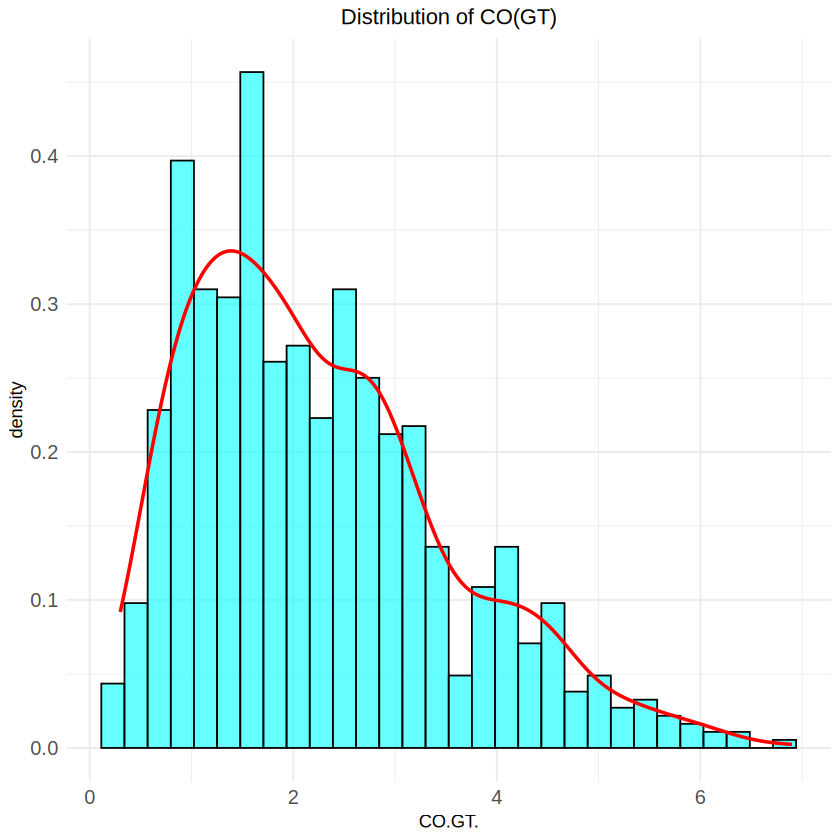
\includegraphics[width=0.75\columnwidth]{air_figures/CO(GT)_original_distribution.png}
    \caption{Phân phối ban đầu của Carbon monoxide.}
    \label{fig:co_original_distribution}
\end{figure}

Nhận xét:
\begin{itemize}
    \item Nhìn vào histogram trên, ta thấy phân phối của biến này bị lệch trái (lệch dương).
\end{itemize}

Ta thử sử dụng log-transform nó.

\begin{figure}[H]
    \centering
    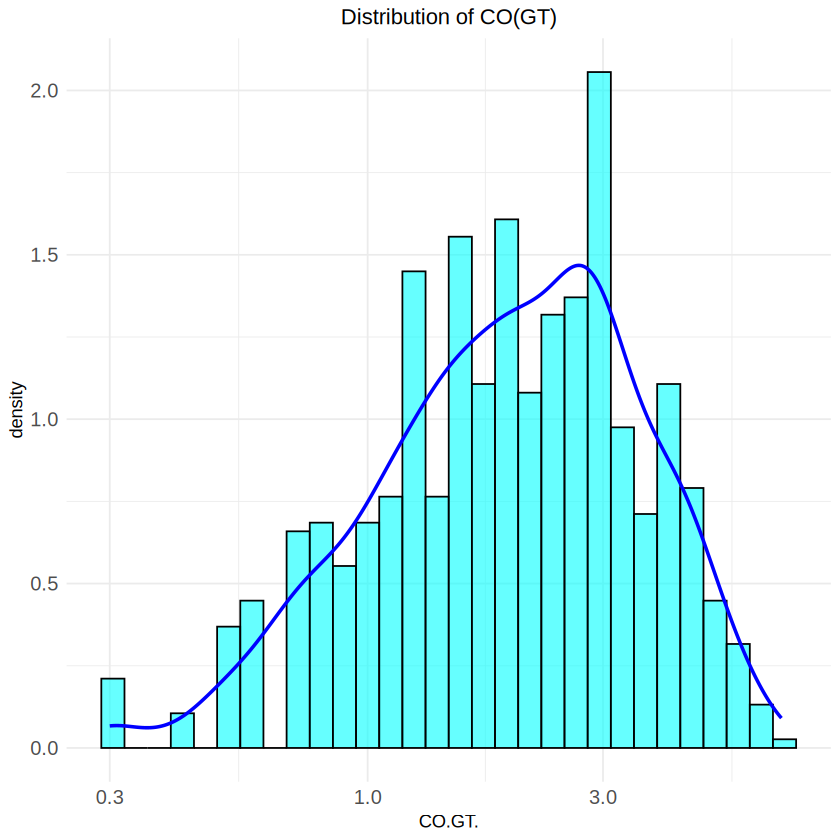
\includegraphics[width=0.75\columnwidth]{air_figures/CO(GT)_logscale_distribution.png}
    \caption{Phân phối sau khi log-scale của Carbon monoxide.}
    \label{fig:co_logscale_distribution}
\end{figure}
Nhận xét:
\begin{itemize}
    \item Sau khi sử dụng log-transform, hình dạng phân phối tương đối chuẩn hơn.
    \item Ta có thể thử sử dụng box-cox transform
\end{itemize}

\begin{figure}[H]
    \centering
    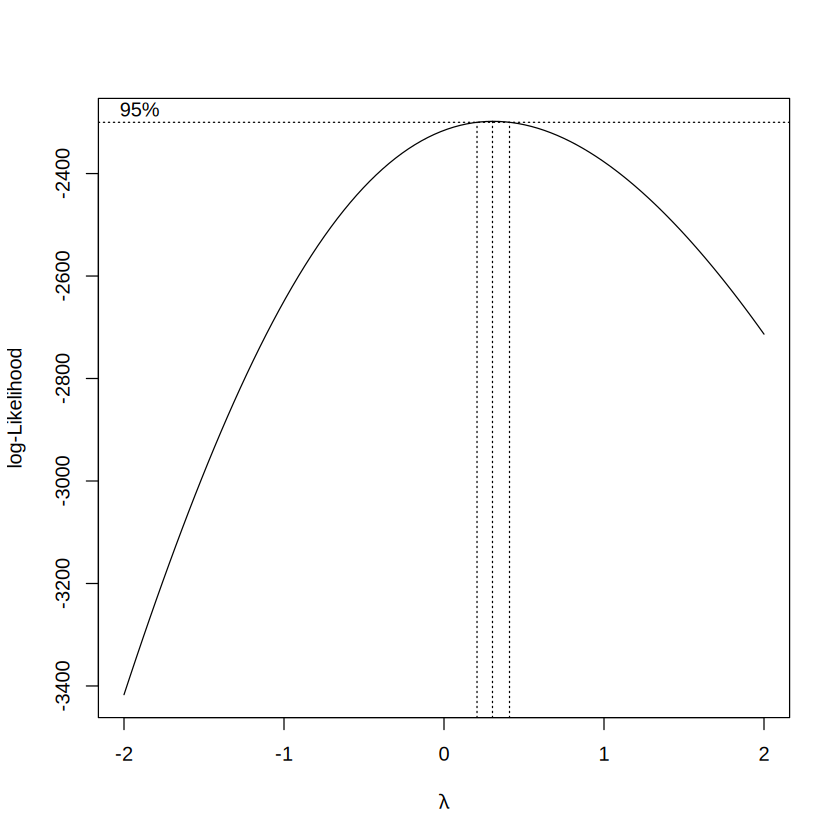
\includegraphics[width=0.75\columnwidth]{air_figures/CO(GT)_optimal_lambda.png}
    \caption{Log-likelihood với các giá trị $\lambda$ của Carbon monoxide.}
    \label{fig:co_optimal_lambda}
\end{figure}
Nhận xét:
\begin{itemize}
    \item Dựa trên biểu đồ, ta tìm được giá trị lambda tối ưu với mức ý nghĩa 5\% là 0.343
\end{itemize}

Và ta thực hiện biến đổi dữ liệu với giá trị lambda vừa tìm được.
\begin{figure}[H]
    \centering
    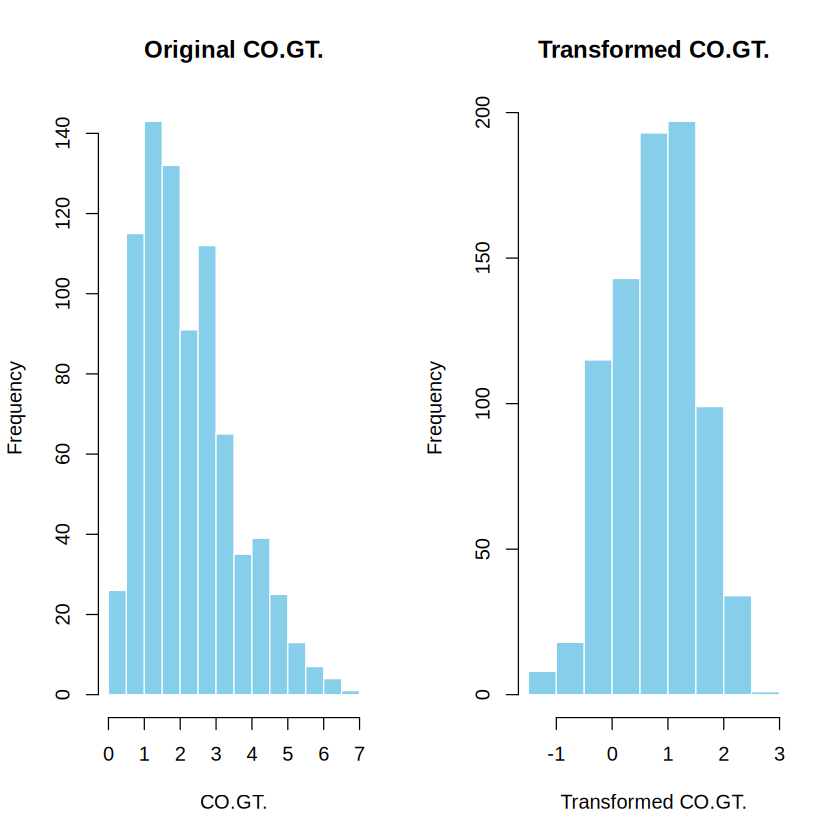
\includegraphics[width=0.75\columnwidth]{air_figures/CO(GT)_transformed_distribution.png}
    \caption{Phân phối trước và sau khi biến đổi của Carbon monoxide.}
    \label{fig:co_transformed_distribution}
\end{figure}
Nhận xét:
\begin{itemize}
    \item Ta có được giá trị lambda tối ưu là 0.343 và sử dụng giá trị này để biến đổi biến CO(GT). Biểu đồ histogram phía bên dưới thể hiện phân phối của biến này trước và sau khi biến đổi. Dễ dàng thấy được, sau khi biến đổi, biến này đã tương đối chuẩn hơn
\end{itemize}

\subsubsection{PT08.S1(CO): Sensor response for CO}

\begin{figure}[H]
    \centering
    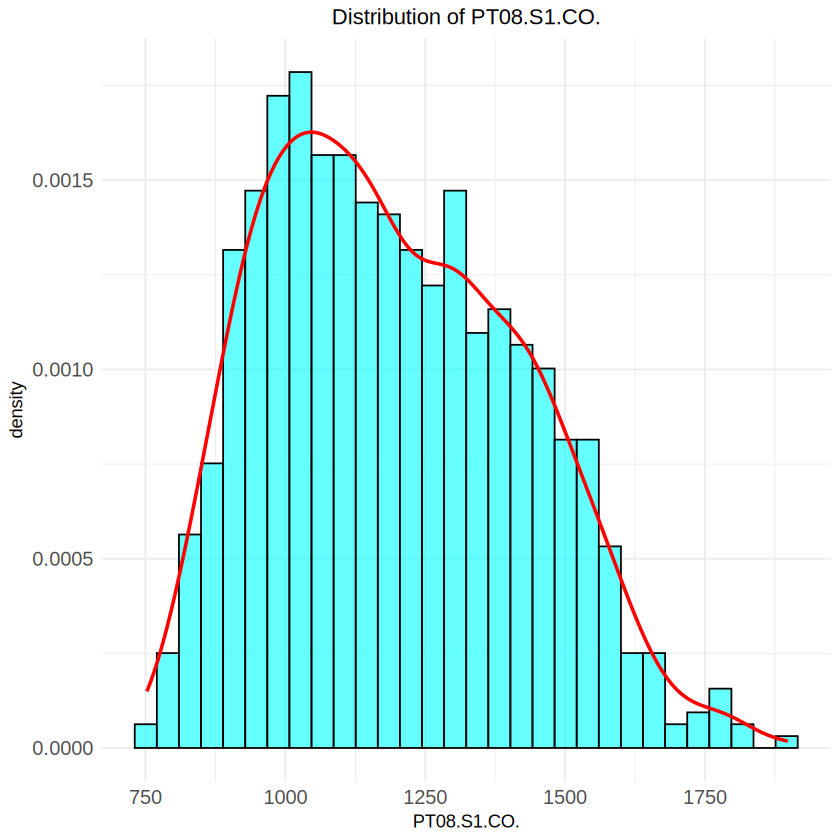
\includegraphics[width=0.75\columnwidth]{air_figures/PT08.S1(CO)_original_distribution.png}
    \caption{Phân phối ban đầu của Sensor response Carbon monoxide.}
    \label{fig:srco_original_distribution}
\end{figure}

Nhận xét:
\begin{itemize}
    \item Nhìn vào histogram trên, ta thấy phân phối của biến này bị lệch trái (lệch dương).
\end{itemize}

Ta thử sử dụng log-transform nó.

\begin{figure}[H]
    \centering
    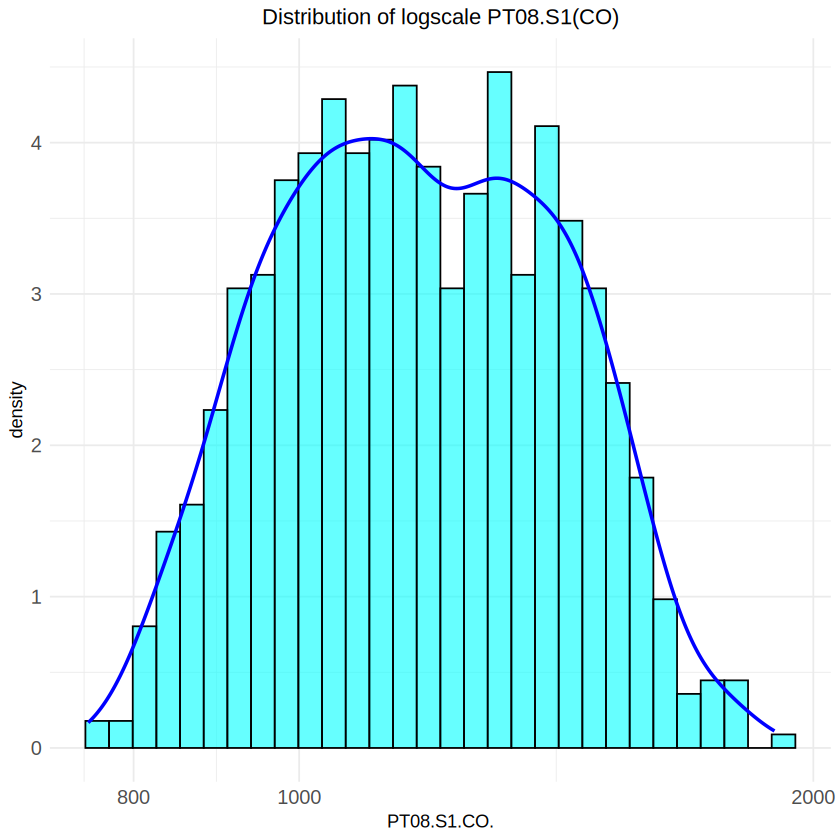
\includegraphics[width=0.75\columnwidth]{air_figures/PT08.S1(CO)_logscale_distribution.png}
    \caption{Phân phối sau khi log-scale của Sensor response Carbon monoxide.}
    \label{fig:srco_logscale_distribution}
\end{figure}
Nhận xét:
\begin{itemize}
    \item Sau khi sử dụng log-transform, hình dạng phân phối tương đối chuẩn hơn.
    \item Ta có thể thử sử dụng box-cox transform
\end{itemize}

\begin{figure}[H]
    \centering
    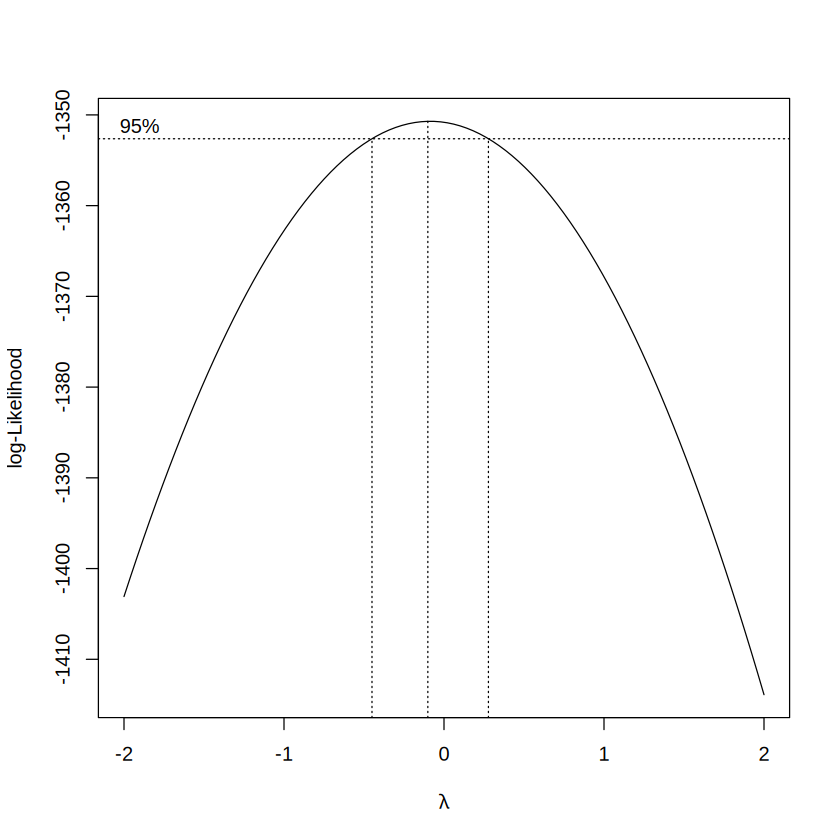
\includegraphics[width=0.75\columnwidth]{air_figures/PT08.S1(CO)_optimal_lambda.png}
    \caption{Log-likelihood với các giá trị $\lambda$ của Sensor response Carbon monoxide.}
    \label{fig:srco_optimal_lambda}
\end{figure}
Nhận xét:
\begin{itemize}
    \item Dựa trên biểu đồ, ta tìm được giá trị lambda tối ưu với mức ý nghĩa 5\% là -0.101
\end{itemize}

Và ta thực hiện biến đổi dữ liệu với giá trị lambda vừa tìm được.
\begin{figure}[H]
    \centering
    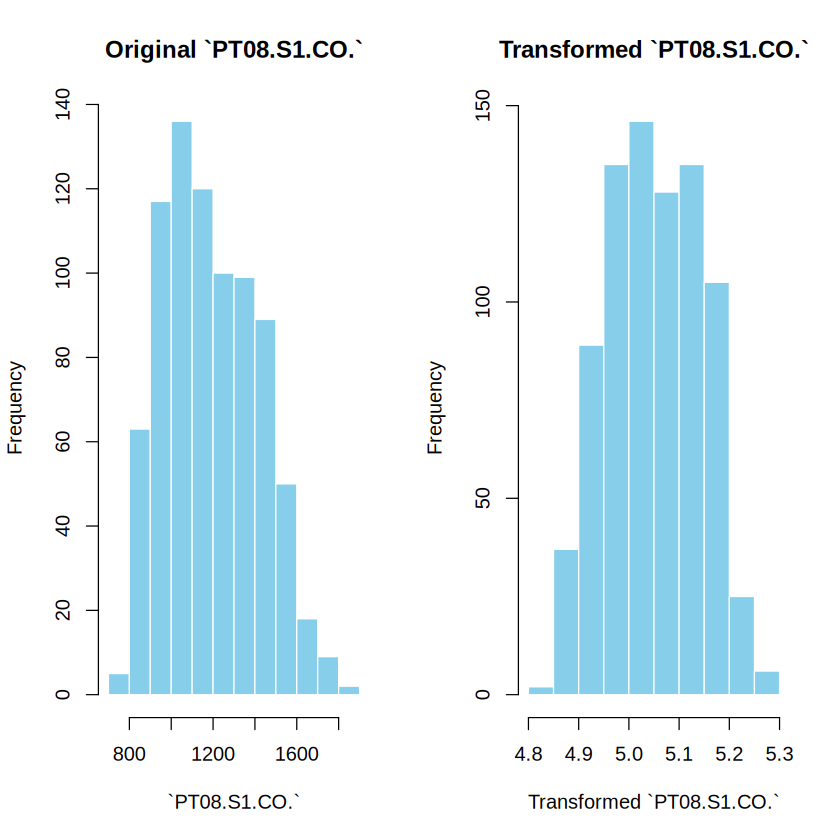
\includegraphics[width=0.75\columnwidth]{air_figures/PT08.S1(CO)_transformed_distribution.png}
    \caption{Phân phối trước và sau khi biến đổi của Sensor response Carbon monoxide.}
    \label{fig:srco_transformed_distribution}
\end{figure}
Nhận xét:
\begin{itemize}
    \item Ta có được giá trị lambda tối ưu là -0.101 và sử dụng giá trị này để biến đổi biến PT08.S1(CO). Biểu đồ histogram phía bên dưới thể hiện phân phối của biến này trước và sau khi biến đổi. Dễ dàng thấy được, sau khi biến đổi, biến này đã tương đối chuẩn hơn.
\end{itemize}

\subsubsection{NMHC(GT): Non-methane hydrocarbons concentration ($\mu g/ m^3$)}

\begin{figure}[H]
    \centering
    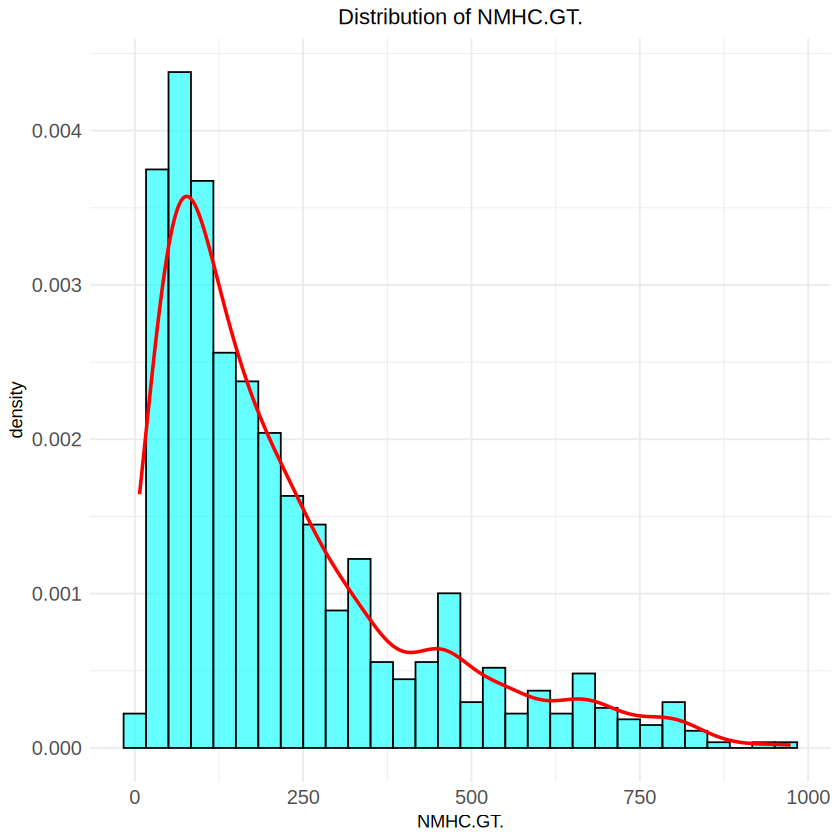
\includegraphics[width=0.75\columnwidth]{air_figures/NMHC(GT)_original_distribution.png}
    \caption{Phân phối ban đầu của Non-methane hydrocarbons.}
    \label{fig:nmhc_original_distribution}
\end{figure}

Nhận xét:
\begin{itemize}
    \item Phân phối tập trung ở giá trị 200
\end{itemize}

Ta thử sử dụng log-transform nó.

\begin{figure}[H]
    \centering
    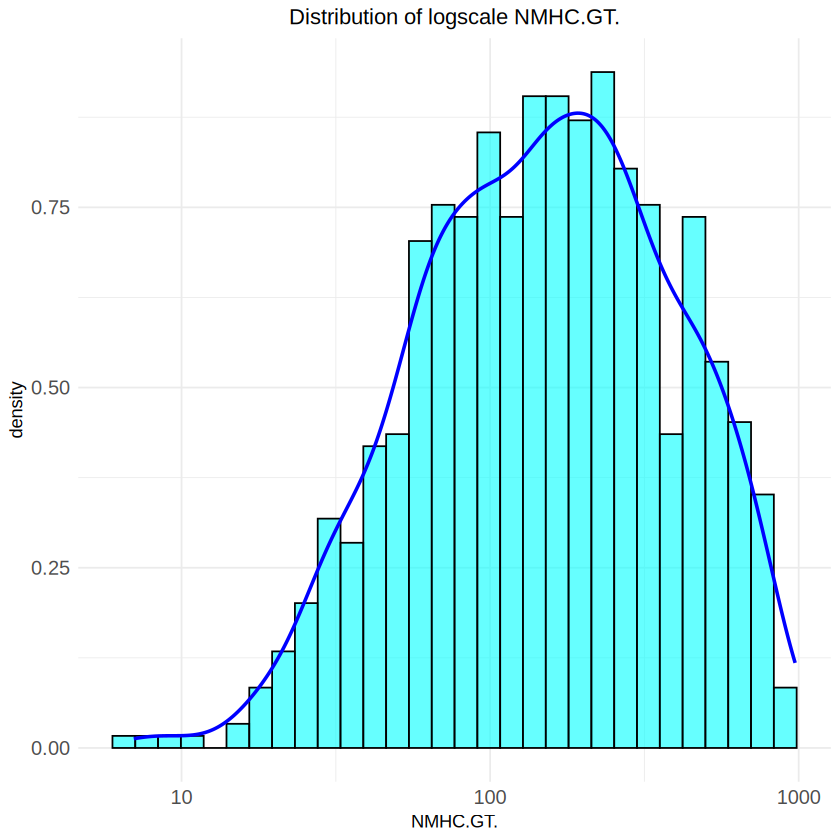
\includegraphics[width=0.75\columnwidth]{air_figures/NMHC(GT)_logscale_distribution.png}
    \caption{Phân phối sau khi log-scale của Non-methane hydrocarbons.}
    \label{fig:nmhc_logscale_distribution}
\end{figure}
Nhận xét:
\begin{itemize}
    \item Nhìn vào histogram trên, ta thấy phân phối của biến này không có nhiều thay đổi.
\end{itemize}

\begin{figure}[H]
    \centering
    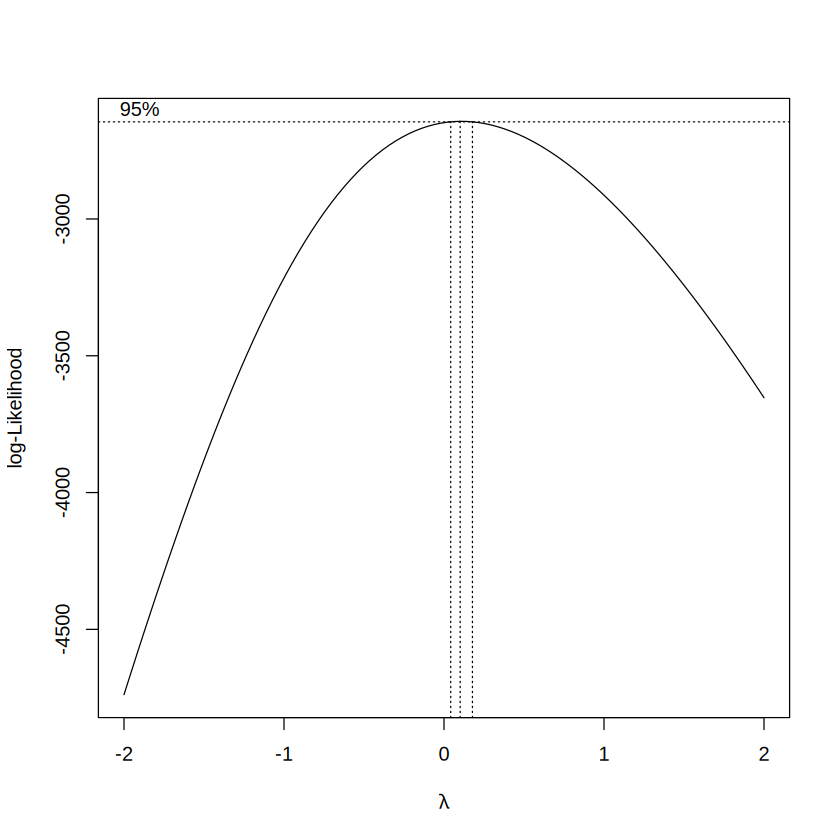
\includegraphics[width=0.75\columnwidth]{air_figures/NMHC(GT)_optimal_lambda.png}
    \caption{Log-likelihood với các giá trị $\lambda$ của Non-methane hydrocarbons.}
    \label{fig:nmhc_optimal_lambda}
\end{figure}
Nhận xét:
\begin{itemize}
    \item Giá trị lambda phù hợp: 0.5858
\end{itemize}

Và ta thực hiện biến đổi dữ liệu với giá trị lambda vừa tìm được.
\begin{figure}[H]
    \centering
    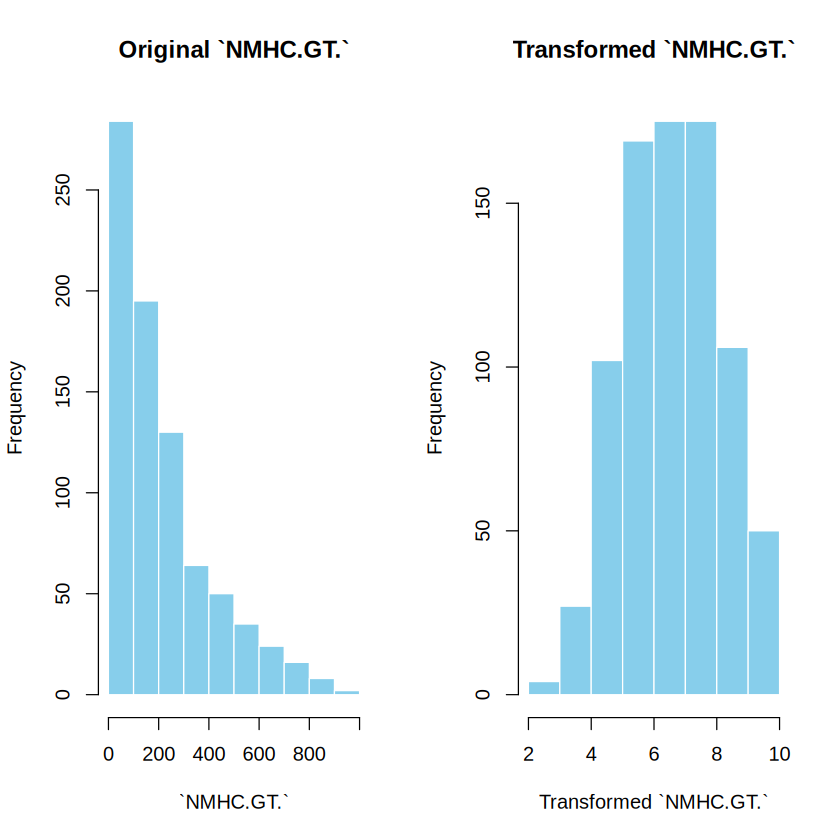
\includegraphics[width=0.75\columnwidth]{air_figures/NMHC(GT)_transformed_distribution.png}
    \caption{Phân phối trước và sau khi biến đổi của Non-methane hydrocarbons}
    \label{fig:nmhc_transformed_distribution}
\end{figure}
Nhận xét:
\begin{itemize}
    \item Sau khi biến đổi, giá trị NMHC(GT) tập trung nhiều ở giá trị 40
\end{itemize}

\subsubsection{C6H6(GT): Benzene concentration ($\mu g/ m^3$)}

\begin{figure}[H]
    \centering
    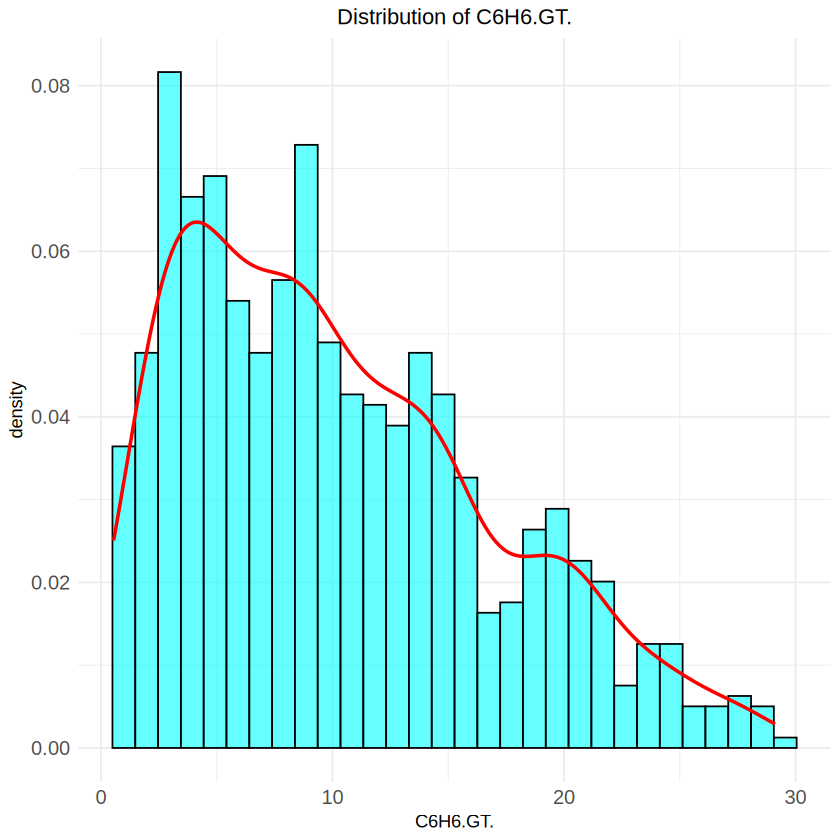
\includegraphics[width=0.75\columnwidth]{air_figures/C6H6(GT)_original_distribution.png}
    \caption{Phân phối ban đầu của Benzene concentration.}
    \label{fig:benzene_original_distribution}
\end{figure}

Nhận xét:
\begin{itemize}
    \item Nhìn vào histogram trên, ta thấy phân phối của biến này bị lệch trái (lệch dương).
\end{itemize}

Ta thử sử dụng log-transform nó.

\begin{figure}[H]
    \centering
    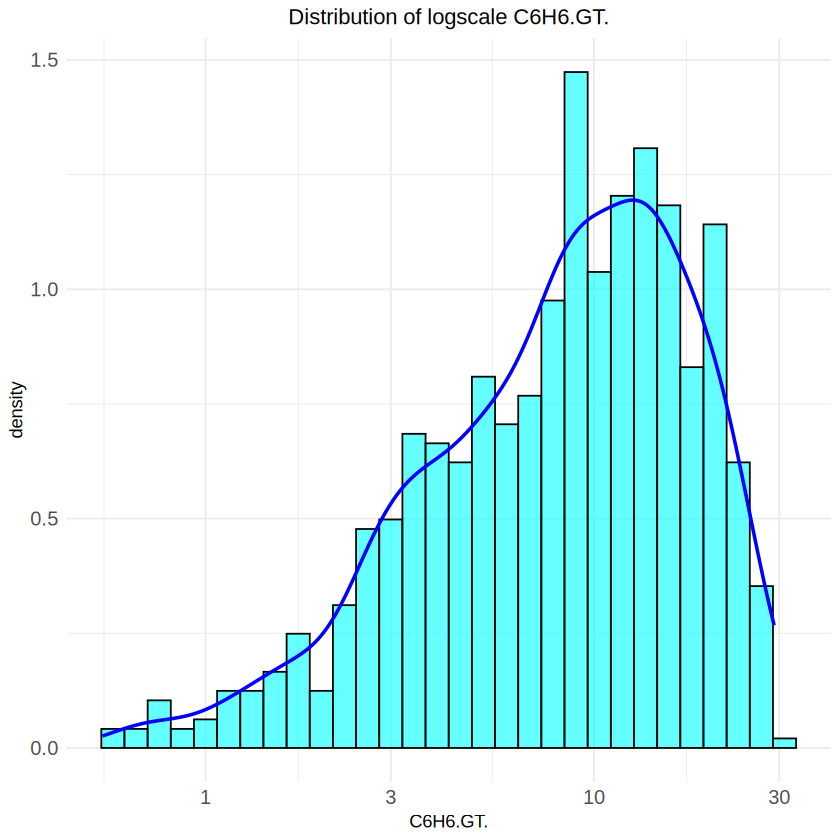
\includegraphics[width=0.75\columnwidth]{air_figures/C6H6(GT)_logscale_distribution.png}
    \caption{Phân phối sau khi log-scale của Non-methane hydrocarbons.}
    \label{fig:benzene_logscale_distribution}
\end{figure}
Nhận xét:
\begin{itemize}
    \item Sau khi sử dụng log-transform, hình dạng phân phối tương đối chuẩn hơn.
    \item Ta có thể thử sử dụng box-cox transform
\end{itemize}

\begin{figure}[H]
    \centering
    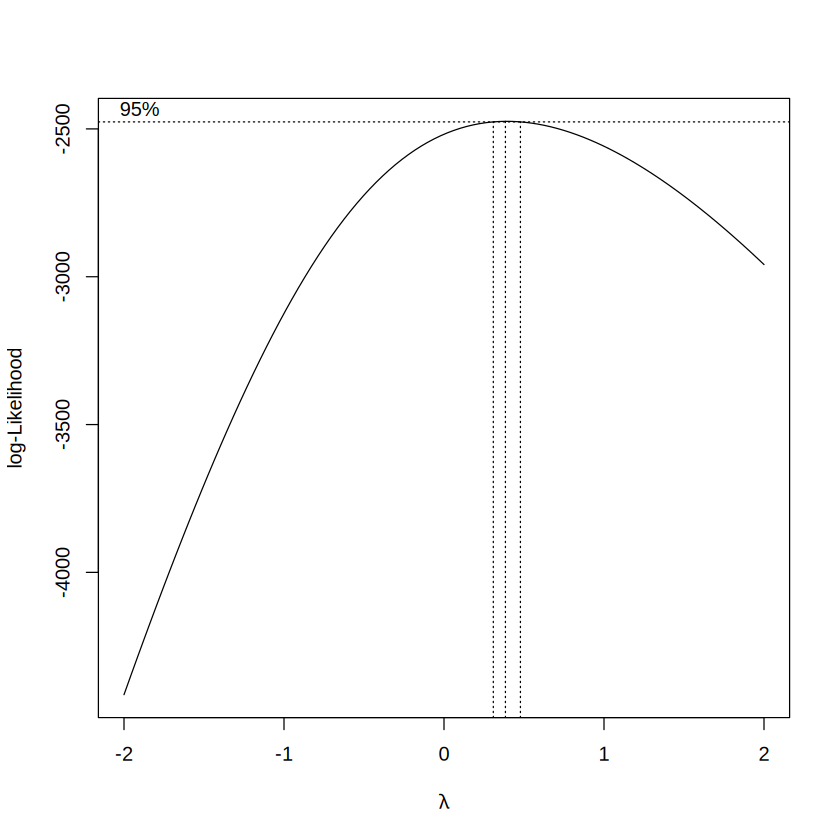
\includegraphics[width=0.75\columnwidth]{air_figures/C6H6(GT)_optimal_lambda.png}
    \caption{Log-likelihood với các giá trị $\lambda$ của Non-methane hydrocarbons.}
    \label{fig:benzene_optimal_lambda}
\end{figure}
Nhận xét:
\begin{itemize}
    \item Giá trị lambda phù hợp: 0.303
\end{itemize}

Và ta thực hiện biến đổi dữ liệu với giá trị lambda vừa tìm được.
\begin{figure}[H]
    \centering
    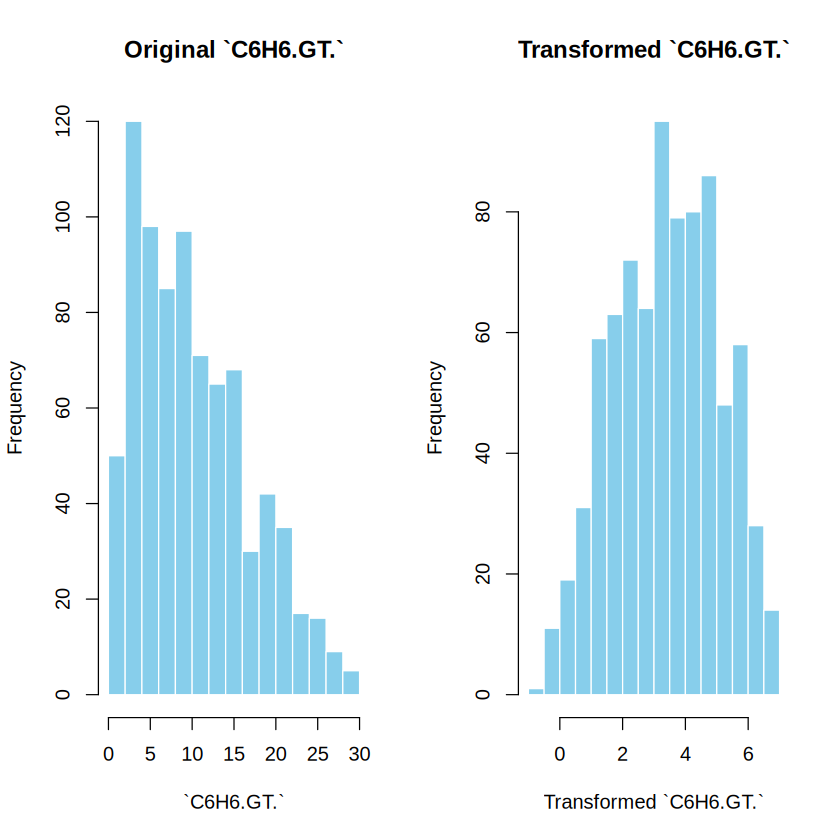
\includegraphics[width=0.75\columnwidth]{air_figures/C6H6(GT)_transformed_distribution.png}
    \caption{Phân phối trước và sau khi biến đổi của Non-methane hydrocarbons}
    \label{fig:benzene_transformed_distribution}
\end{figure}
Nhận xét:
\begin{itemize}
    \item Ta có được giá trị lambda tối ưu là 0.303 và sử dụng giá trị này để biến đổi biến C6H6(GT). Biểu đồ histogram phía bên dưới thể hiện phân phối của biến này trước và sau khi biến đổi. Dễ dàng thấy được, sau khi biến đổi, biến này đã tương đối chuẩn hơn.
\end{itemize}

\subsubsection{PT08.S2(NMHC): Sensor response for NMHC}

\begin{figure}[H]
    \centering
    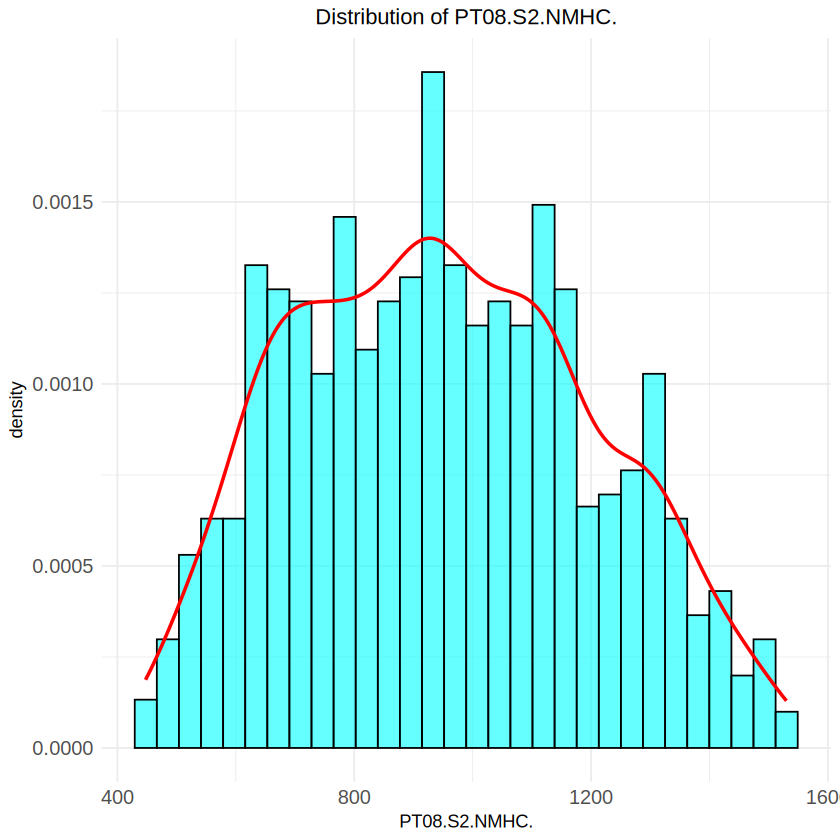
\includegraphics[width=0.75\columnwidth]{air_figures/PT08.S2(NMHC)_original_distribution.png}
    \caption{Phân phối ban đầu của Sensor response cho NMHC.}
    \label{fig:srnmhc_original_distribution}
\end{figure}

Nhận xét:
\begin{itemize}
    \item Nhìn vào histogram trên, ta thấy phân phối của biến này tương đối chuẩn.
    \item Tuy nhiên, cẩn thận hơn, ta cũng chuẩn hóa biến này.
\end{itemize}

Ta thử sử dụng log-transform nó.

\begin{figure}[H]
    \centering
    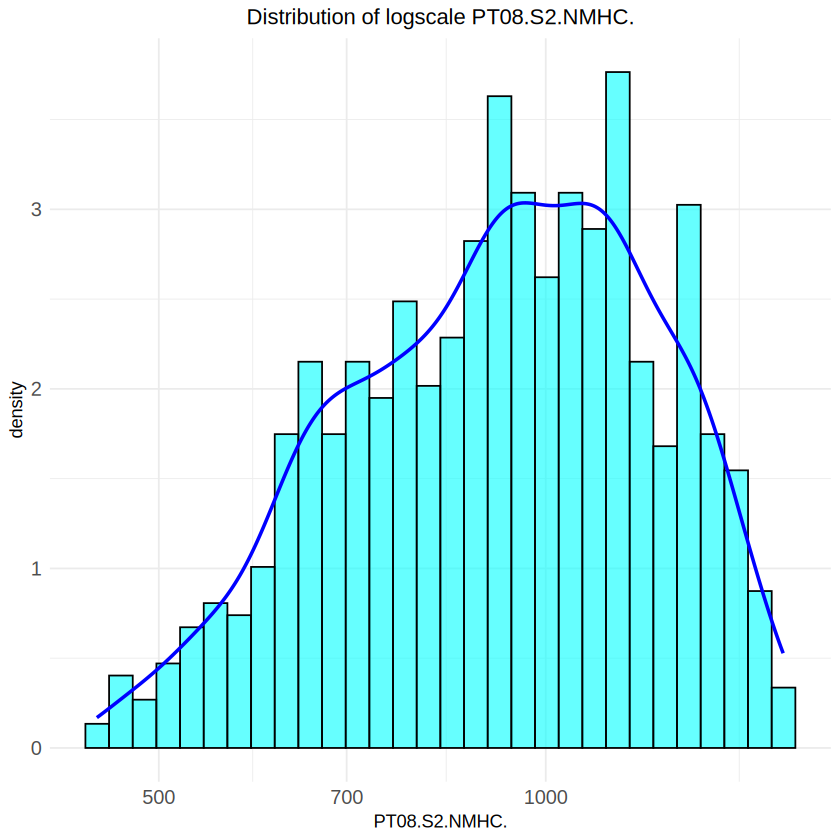
\includegraphics[width=0.75\columnwidth]{air_figures/PT08.S2(NMHC)_logscale_distribution.png}
    \caption{Phân phối sau khi log-scale của Sensor response cho NMHC.}
    \label{fig:srnmhc_logscale_distribution}
\end{figure}
Nhận xét:
\begin{itemize}
    \item Sau khi log-transform, ta thấy phân phối của biến bị lệch trái. 
    \item Ta cần sử dụng box-cox để tìm giá trị biến đổi phù hợp cho nó.
\end{itemize}

\begin{figure}[H]
    \centering
    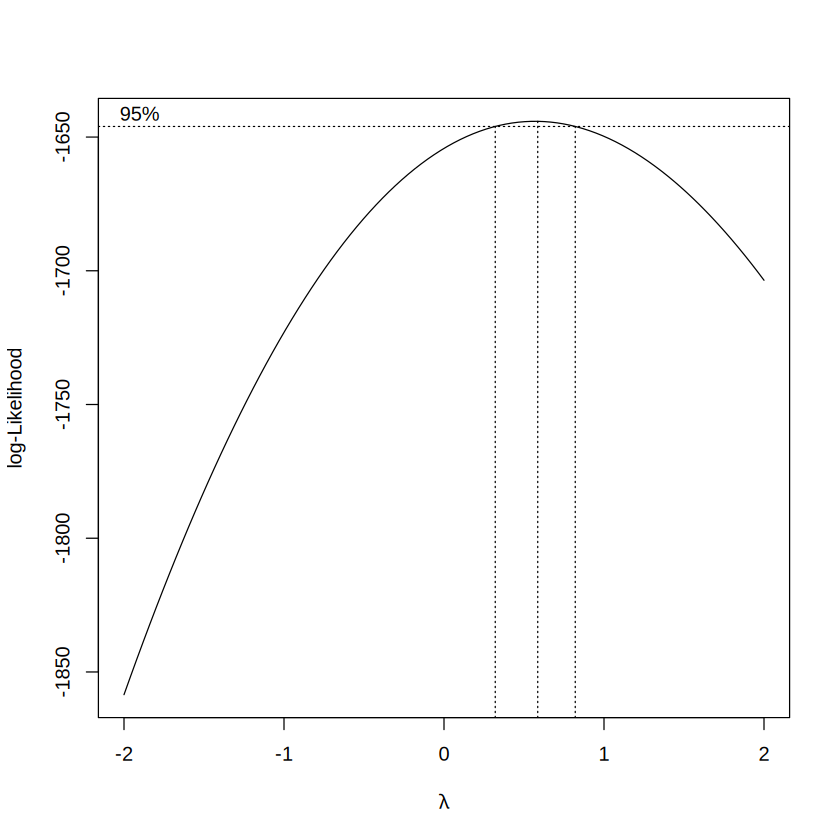
\includegraphics[width=0.75\columnwidth]{air_figures/PT08.S2(NMHC)_optimal_lambda.png}
    \caption{Log-likelihood với các giá trị $\lambda$ của Sensor response cho NMHC.}
    \label{fig:srnmhc_optimal_lambda}
\end{figure}
Nhận xét:
\begin{itemize}
    \item Giá trị lambda phù hợp với mức ý nghĩa 5\% là 0.18181
\end{itemize}

Và ta thực hiện biến đổi dữ liệu với giá trị lambda vừa tìm được.
\begin{figure}[H]
    \centering
    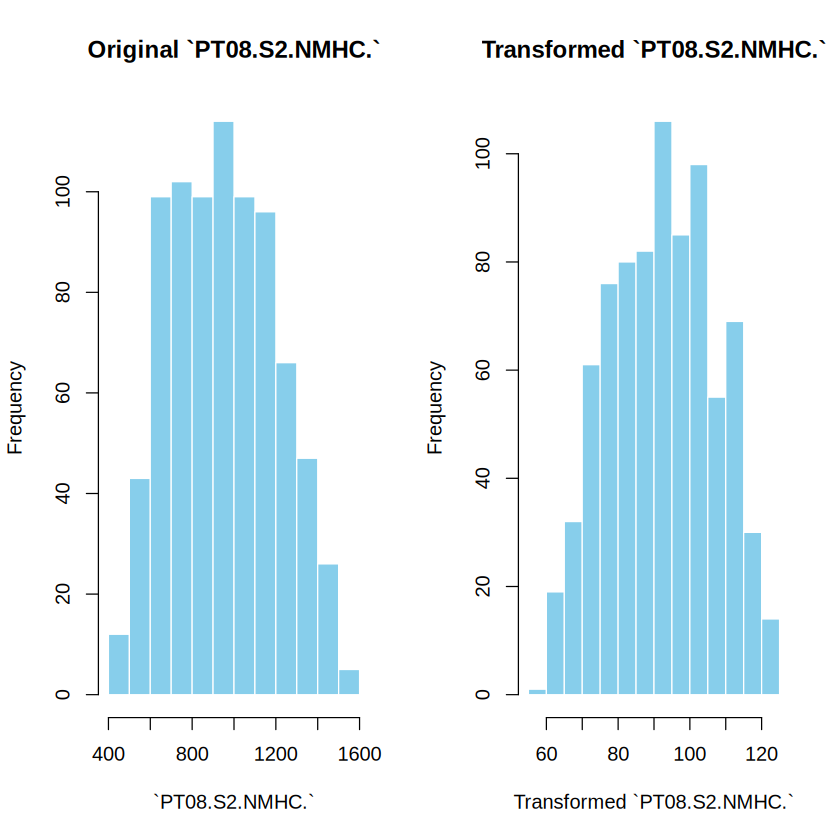
\includegraphics[width=0.75\columnwidth]{air_figures/PT08.S2(NMHC)_transformed_distribution.png}
    \caption{Phân phối trước và sau khi biến đổi của Sensor response cho NMHC}
    \label{fig:srnmhc_transformed_distribution}
\end{figure}
Nhận xét:
\begin{itemize}
    \item Ta có được giá trị lambda tối ưu là 0.18181 và sử dụng giá trị này để biến đổi biến PT08.S2(NMHC). Biểu đồ histogram phía bên dưới thể hiện phân phối của biến này trước và sau khi biến đổi. Dễ dàng thấy được, sau khi biến đổi, biến này đã tương đối chuẩn hơn.
\end{itemize}

\subsubsection{NOx(GT): Nitrogen oxides concentration (ppb)}

\begin{figure}[H]
    \centering
    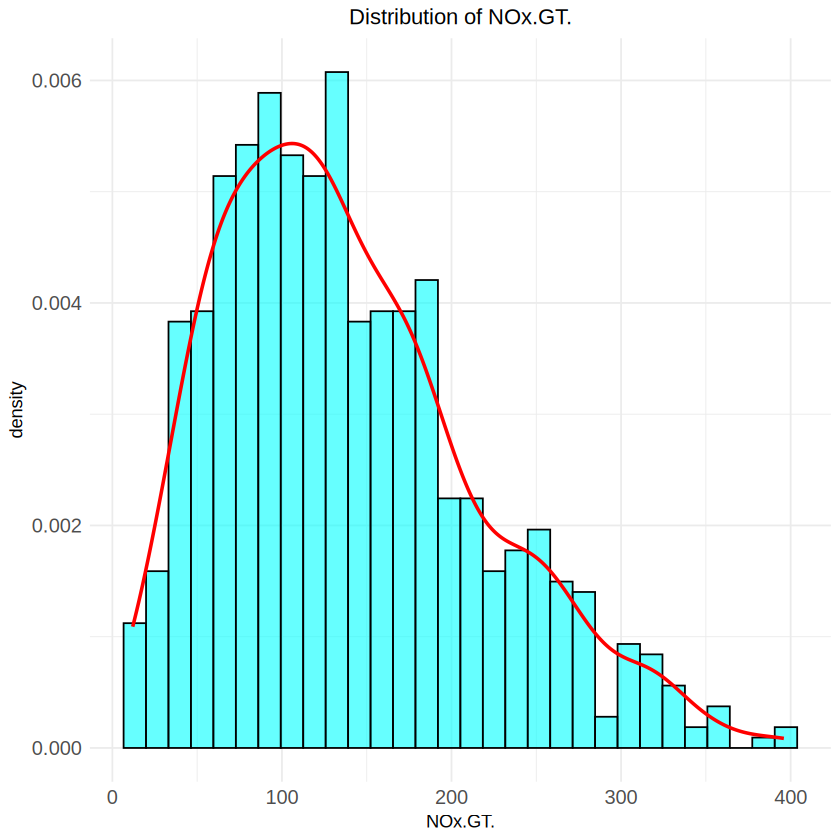
\includegraphics[width=0.75\columnwidth]{air_figures/NOx(GT)_original_distribution.png}
    \caption{Phân phối ban đầu của Sensor response cho Nitrogen oxides.}
    \label{fig:nox_original_distribution}
\end{figure}

Nhận xét:
\begin{itemize}
    \item Nhìn vào histogram trên, ta thấy phân phối của biến này bị lệch trái (lệch dương).
\end{itemize}

Ta thử sử dụng log-transform nó.

\begin{figure}[H]
    \centering
    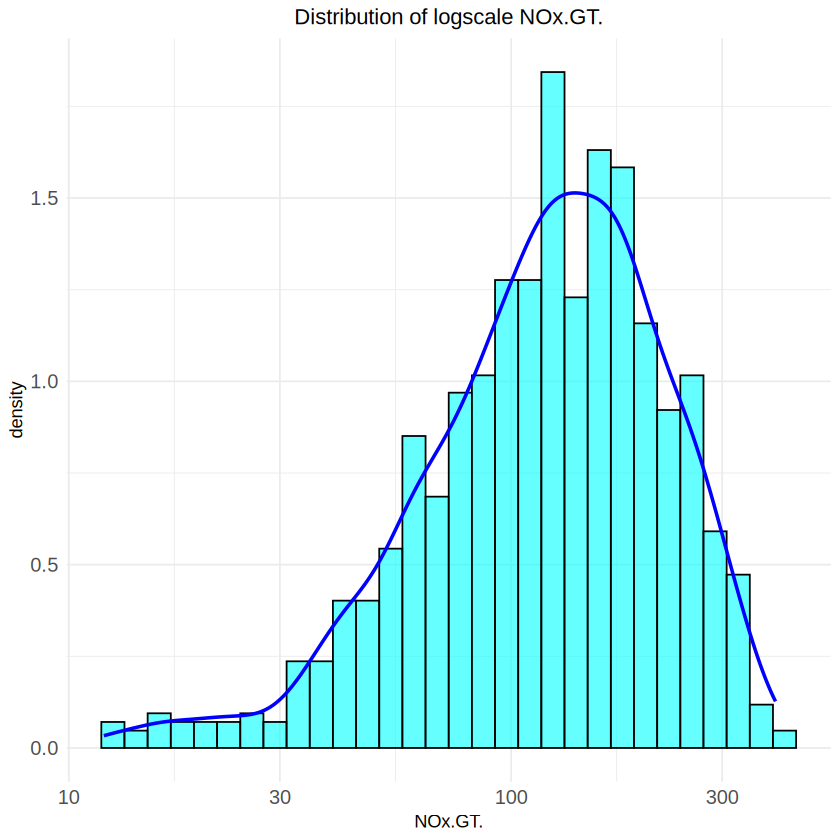
\includegraphics[width=0.75\columnwidth]{air_figures/NOx(GT)_logscale_distribution.png}
    \caption{Phân phối sau khi log-scale của Sensor response cho Nitrogen oxides.}
    \label{fig:nox_logscale_distribution}
\end{figure}
Nhận xét:
\begin{itemize}
    \item Sau khi logscale, ta thấy phân phối có chiều hướng lệch phải (lệch âm)
    \item Ta cần sử dụng box-cox
\end{itemize}

\begin{figure}[H]
    \centering
    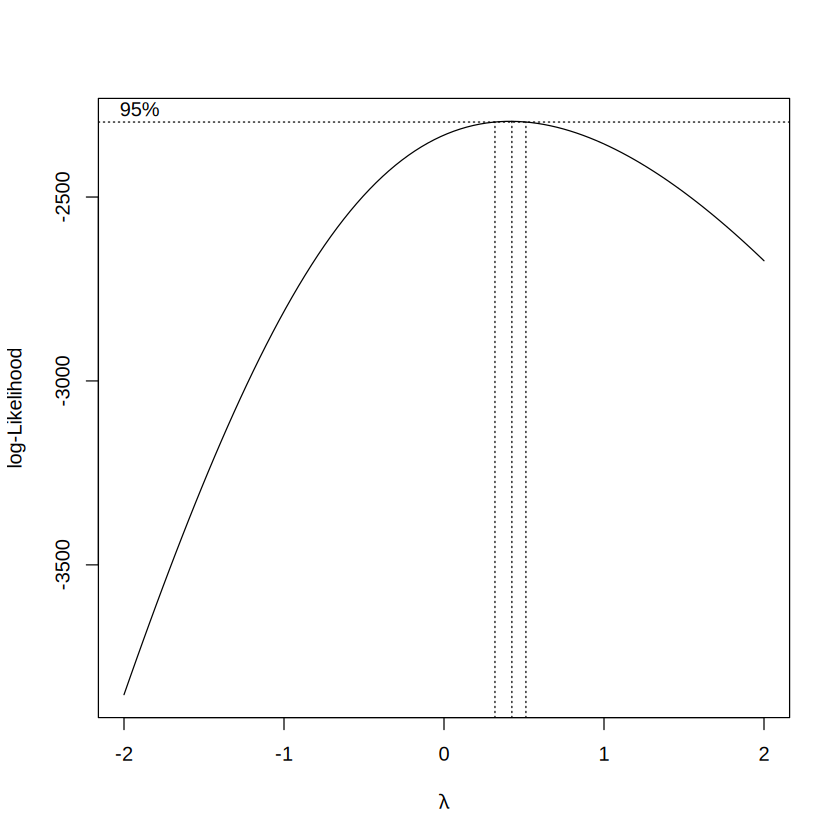
\includegraphics[width=0.75\columnwidth]{air_figures/NOx(GT)_optimal_lambda.png}
    \caption{Log-likelihood với các giá trị $\lambda$ của Sensor response cho Nitrogen oxides.}
    \label{fig:nox_optimal_lambda}
\end{figure}
Nhận xét:
\begin{itemize}
    \item Với mức ý nghĩa 5\%, ta tìm được giá trị lambda phù hợp là 0.2222
\end{itemize}

Và ta thực hiện biến đổi dữ liệu với giá trị lambda vừa tìm được.
\begin{figure}[H]
    \centering
    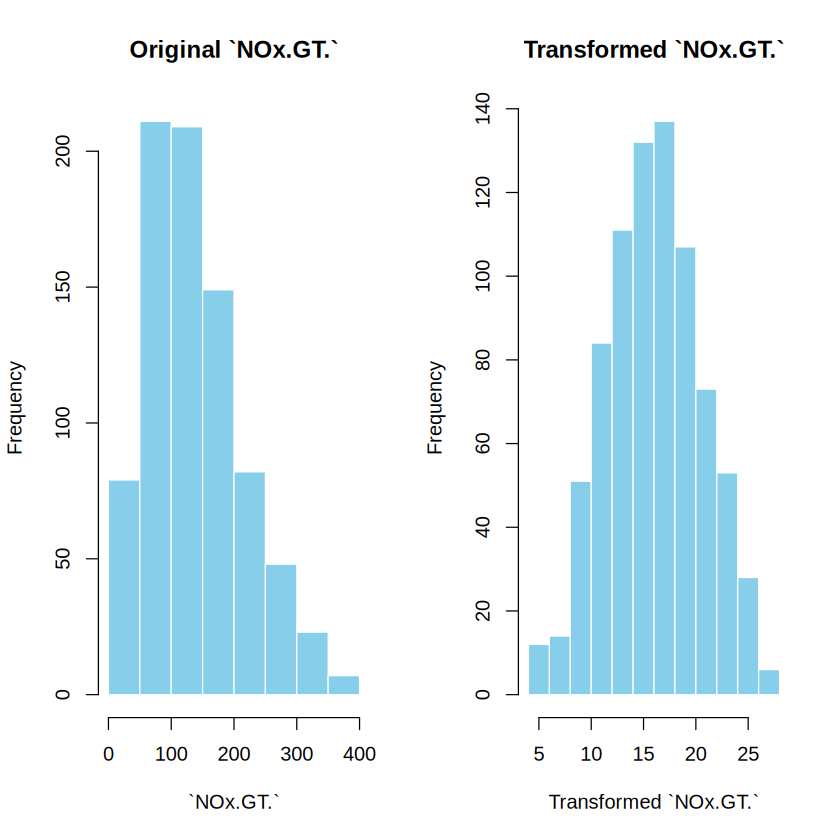
\includegraphics[width=0.75\columnwidth]{air_figures/NOx(GT)_transformed_distribution.png}
    \caption{Phân phối trước và sau khi biến đổi của Sensor response cho Nitrogen oxides.}
    \label{fig:nox_transformed_distribution}
\end{figure}
Nhận xét:
\begin{itemize}
    \item Ta có được giá trị lambda tối ưu là 0.2222 và sử dụng giá trị này để biến đổi biến NOx(GT). Biểu đồ histogram phía bên dưới thể hiện phân phối của biến này trước và sau khi biến đổi. Dễ dàng thấy được, sau khi biến đổi, biến này đã tương đối chuẩn hơn.
\end{itemize}

\subsubsection{PT08.S3(NOx): Sensor response for NOx}

\begin{figure}[H]
    \centering
    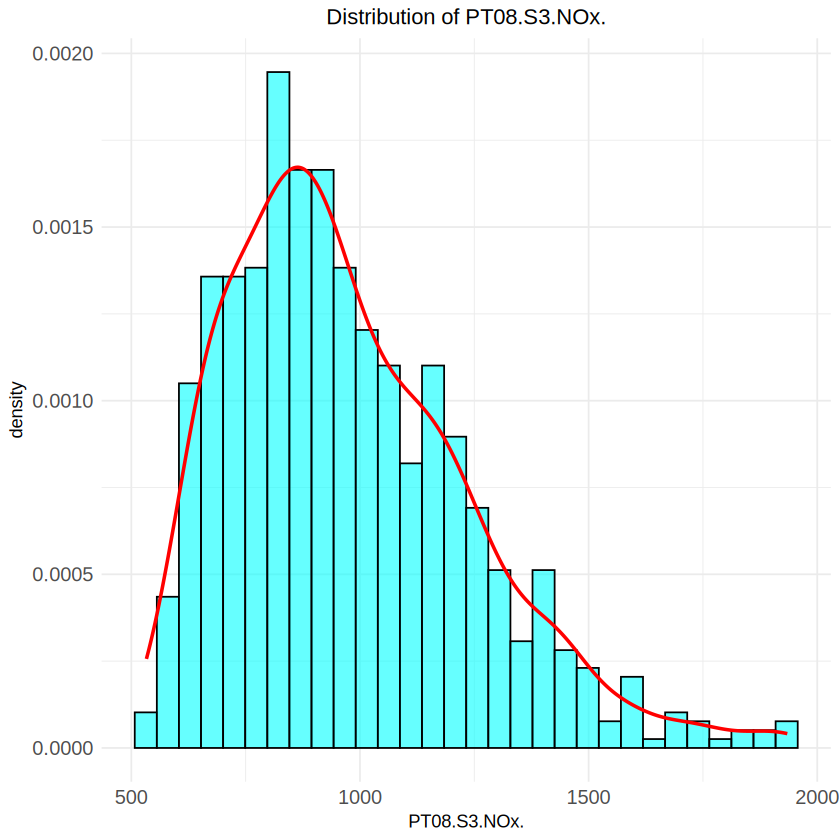
\includegraphics[width=0.75\columnwidth]{air_figures/PT08.S3(NOx)_original_distribution.png}
    \caption{Phân phối ban đầu của Sensor response cho Nitrogen oxides.}
    \label{fig:ptnox_original_distribution}
\end{figure}

Nhận xét:
\begin{itemize}
    \item Nhìn vào histogram trên, ta thấy phân phối của biến này bị lệch trái (lệch dương).
\end{itemize}

Ta thử sử dụng log-transform nó.

\begin{figure}[H]
    \centering
    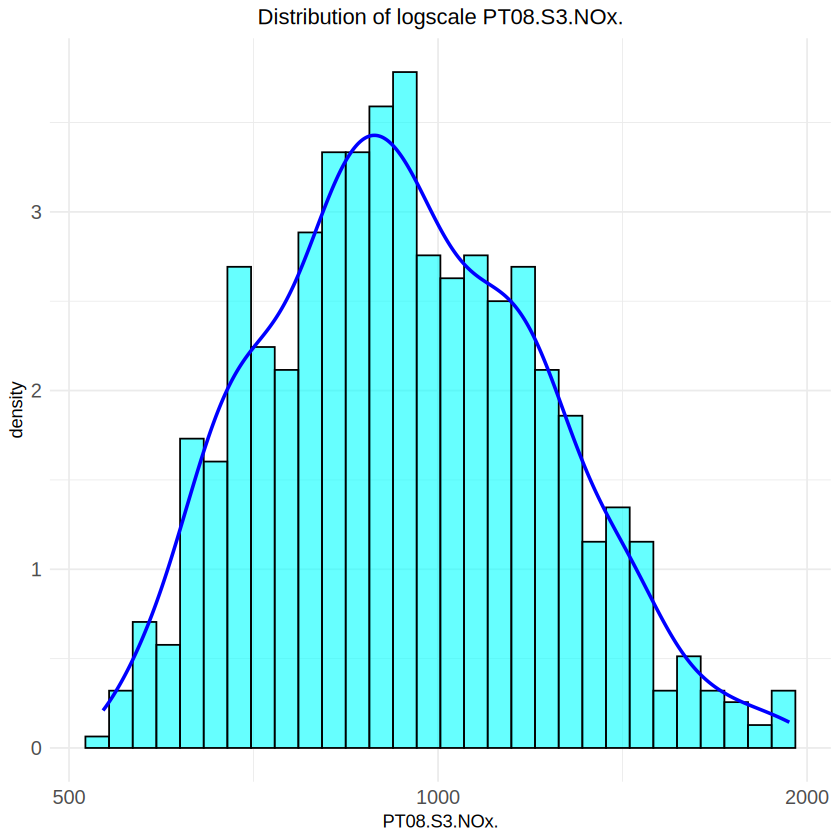
\includegraphics[width=0.75\columnwidth]{air_figures/PT08.S3(NOx)_logscale_distribution.png}
    \caption{Phân phối sau khi log-scale của Sensor response cho Nitrogen oxides.}
    \label{fig:ptnox_logscale_distribution}
\end{figure}
Nhận xét:
\begin{itemize}
    \item Sau khi logscale, ta thấy phân phối của biến này xấp xỉ chuẩn hơn
\end{itemize}

\begin{figure}[H]
    \centering
    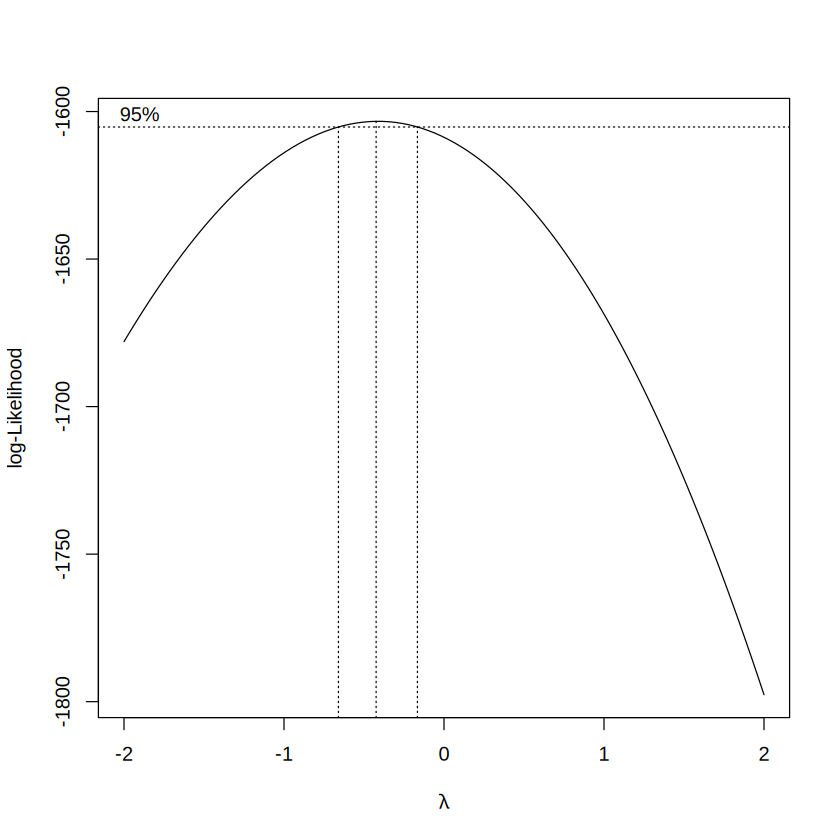
\includegraphics[width=0.75\columnwidth]{air_figures/PT08.S3(NOx)_optimal_lambda.png}
    \caption{Log-likelihood với các giá trị $\lambda$ của Sensor response cho Nitrogen oxides.}
    \label{fig:ptnox_optimal_lambda}
\end{figure}
Nhận xét:
\begin{itemize}
    \item Với mức ý nghĩa 5\%, ta tìm được giá trị lambda phù hợp là -0.02020
\end{itemize}

Và ta thực hiện biến đổi dữ liệu với giá trị lambda vừa tìm được.
\begin{figure}[H]
    \centering
    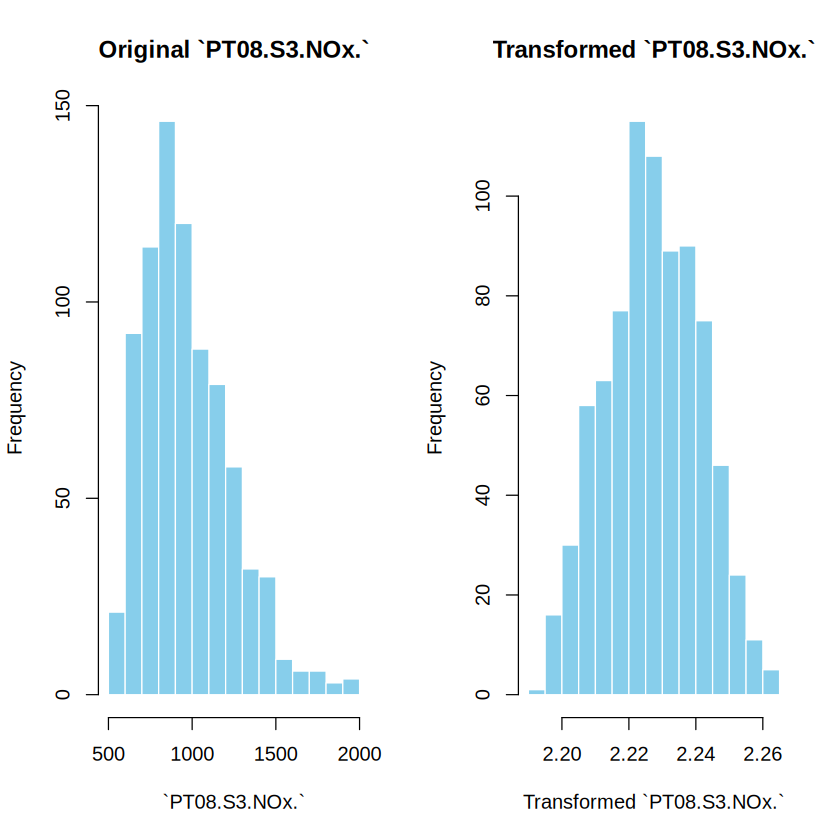
\includegraphics[width=0.75\columnwidth]{air_figures/PT08.S3(NOx)_transformed_distribution.png}
    \caption{Phân phối trước và sau khi biến đổi của Sensor response cho Nitrogen oxides.}
    \label{fig:ptnox_transformed_distribution}
\end{figure}
Nhận xét:
\begin{itemize}
    \item Ta có được giá trị lambda tối ưu là -0.02020 và sử dụng giá trị này để biến đổi biến PT08.S3(NOx). Biểu đồ histogram phía bên dưới thể hiện phân phối của biến này trước và sau khi biến đổi. Dễ dàng thấy được, sau khi biến đổi, biến này đã tương đối chuẩn hơn.
\end{itemize}

\subsubsection{NO2(GT): Nitrogen dioxide concentration ($\mu g/ m^3$)}

\begin{figure}[H]
    \centering
    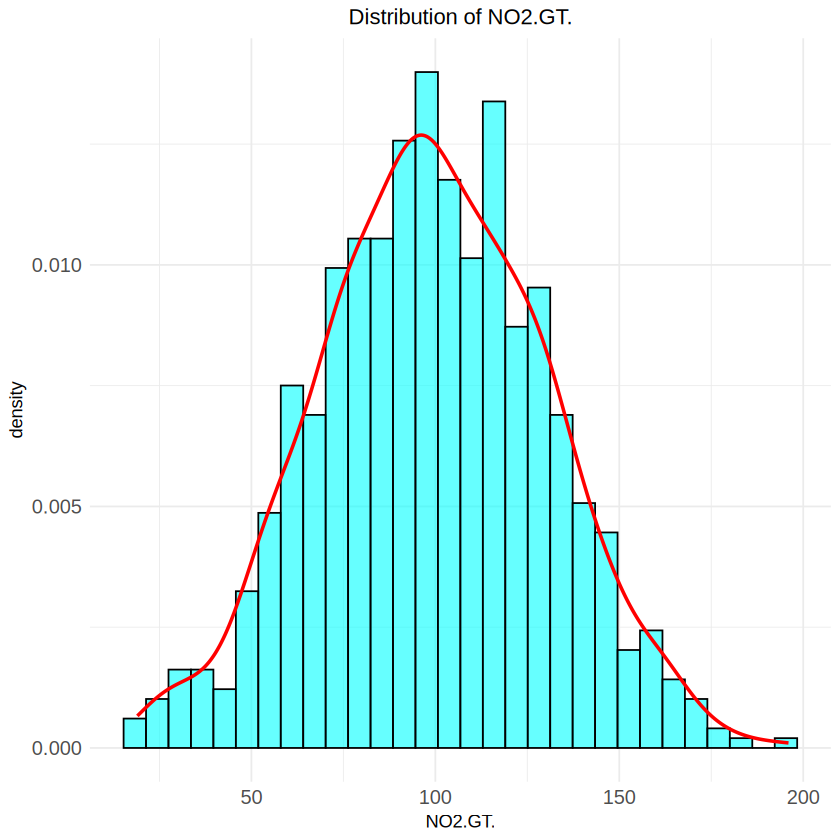
\includegraphics[width=0.75\columnwidth]{air_figures/NO2(GT)_original_distribution.png}
    \caption{Phân phối ban đầu của Sensor response cho Nitrogen oxides.}
    \label{fig:no2_original_distribution}
\end{figure}

Nhận xét:
\begin{itemize}
    \item Nhìn vào histogram trên, ta thấy phân phối của biến này xấp xỉ chuẩn.
\end{itemize}

Ta thử sử dụng log-transform nó.

\begin{figure}[H]
    \centering
    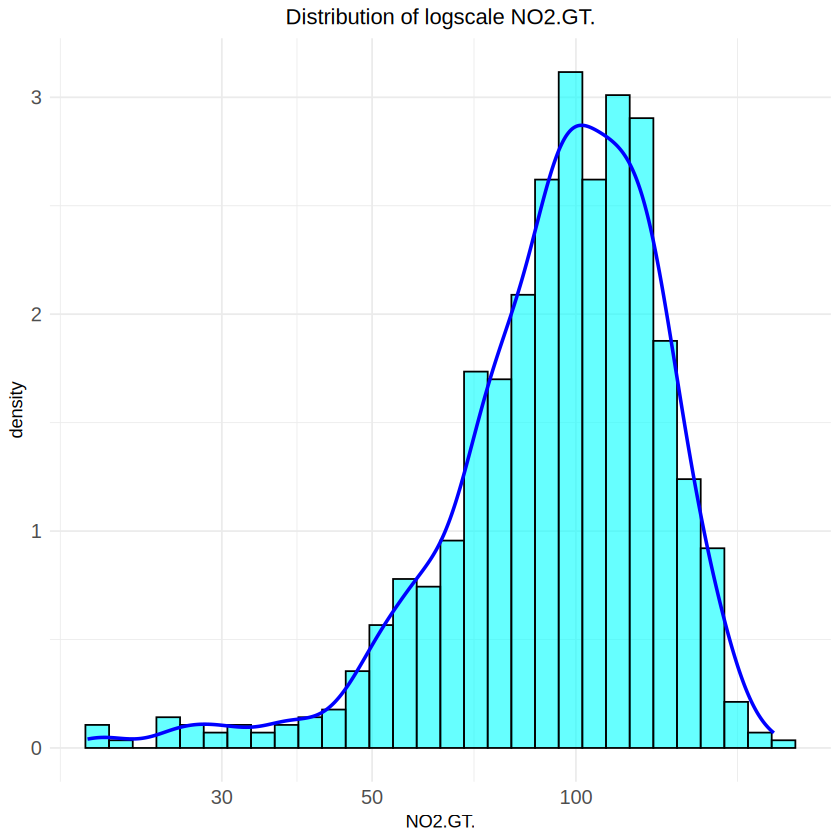
\includegraphics[width=0.75\columnwidth]{air_figures/NO2(GT)_logscale_distribution.png}
    \caption{Phân phối sau khi log-scale của Sensor response cho Nitrogen oxides.}
    \label{fig:no2_logscale_distribution}
\end{figure}
Nhận xét:
\begin{itemize}
    \item Sau khi logscale, ta thấy phân phối của biến này có chiều hướng lệch phải (lệch âm)
\end{itemize}

\begin{figure}[H]
    \centering
    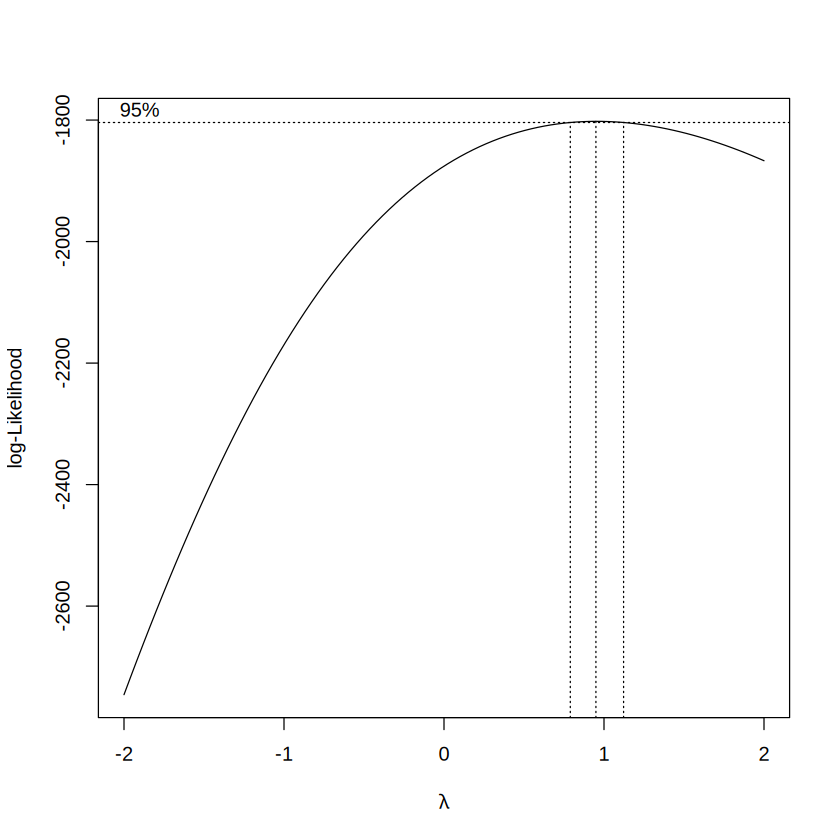
\includegraphics[width=0.75\columnwidth]{air_figures/NO2(GT)_optimal_lambda.png}
    \caption{Log-likelihood với các giá trị $\lambda$ của Sensor response cho Nitrogen oxides.}
    \label{fig:no2_optimal_lambda}
\end{figure}
Nhận xét:
\begin{itemize}
    \item Với mức ý nghĩa 5\%, ta tìm được giá trị lambda phù hợp 0.58585
\end{itemize}

Và ta thực hiện biến đổi dữ liệu với giá trị lambda vừa tìm được.
\begin{figure}[H]
    \centering
    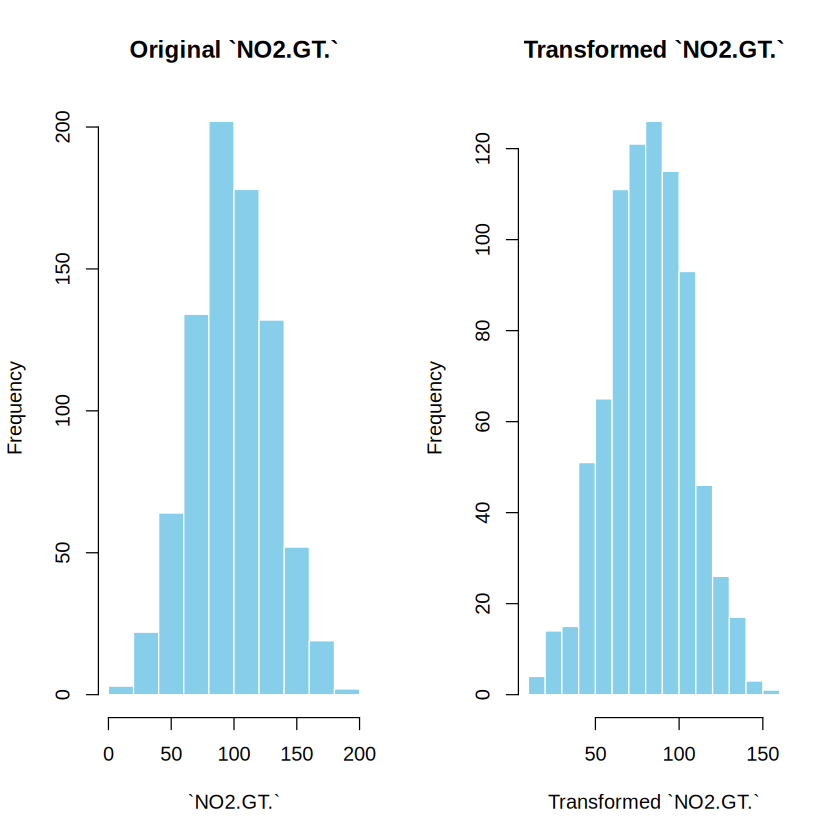
\includegraphics[width=0.75\columnwidth]{air_figures/NO2(GT)_transformed_distribution.png}
    \caption{Phân phối trước và sau khi biến đổi của Sensor response cho Nitrogen oxides.}
    \label{fig:no2_transformed_distribution}
\end{figure}
Nhận xét:
\begin{itemize}
    \item Ta có được giá trị lambda tối ưu là 0.58585 và sử dụng giá trị này để biến đổi biến NO2(GT)). Biểu đồ histogram phía bên dưới thể hiện phân phối của biến này trước và sau khi biến đổi. Dễ dàng thấy được, sau khi biến đổi, biến này đã tương đối chuẩn hơn.
\end{itemize}

\subsubsection{PT08.S4(NO2): Sensor response for NO2}

\begin{figure}[H]
    \centering
    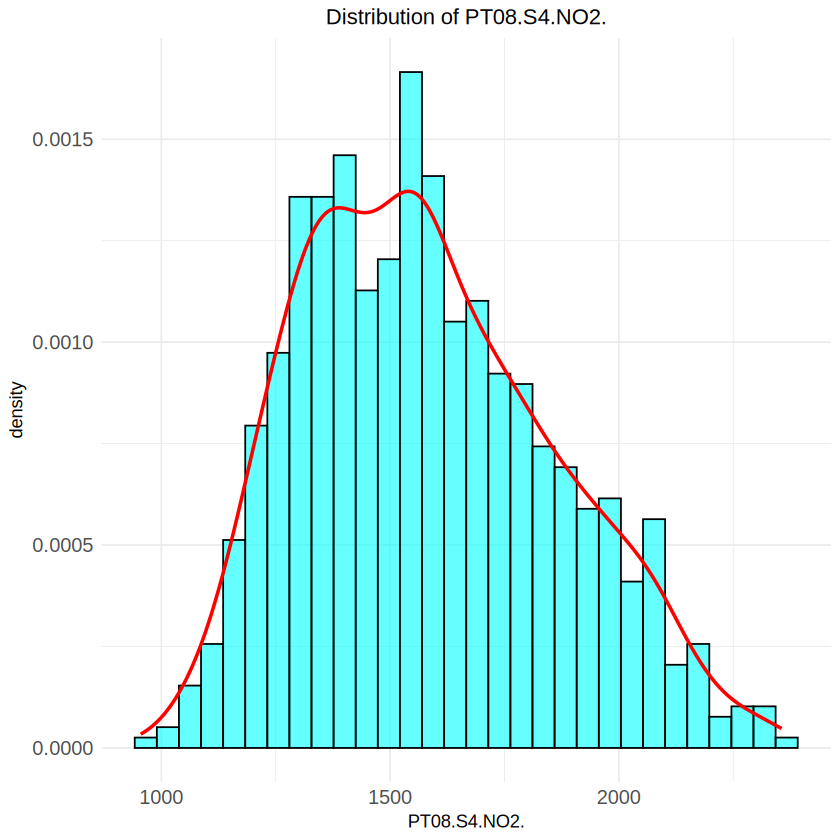
\includegraphics[width=0.75\columnwidth]{air_figures/PT08.S4(NO2)_original_distribution.png}
    \caption{Phân phối ban đầu của Sensor response cho Nitrogen oxides.}
    \label{fig:ptno2_original_distribution}
\end{figure}

Nhận xét:
\begin{itemize}
    \item Nhìn vào histogram trên, ta thấy phân phối của biến này xấp xỉ chuẩn.
\end{itemize}

Ta thử sử dụng log-transform nó.

\begin{figure}[H]
    \centering
    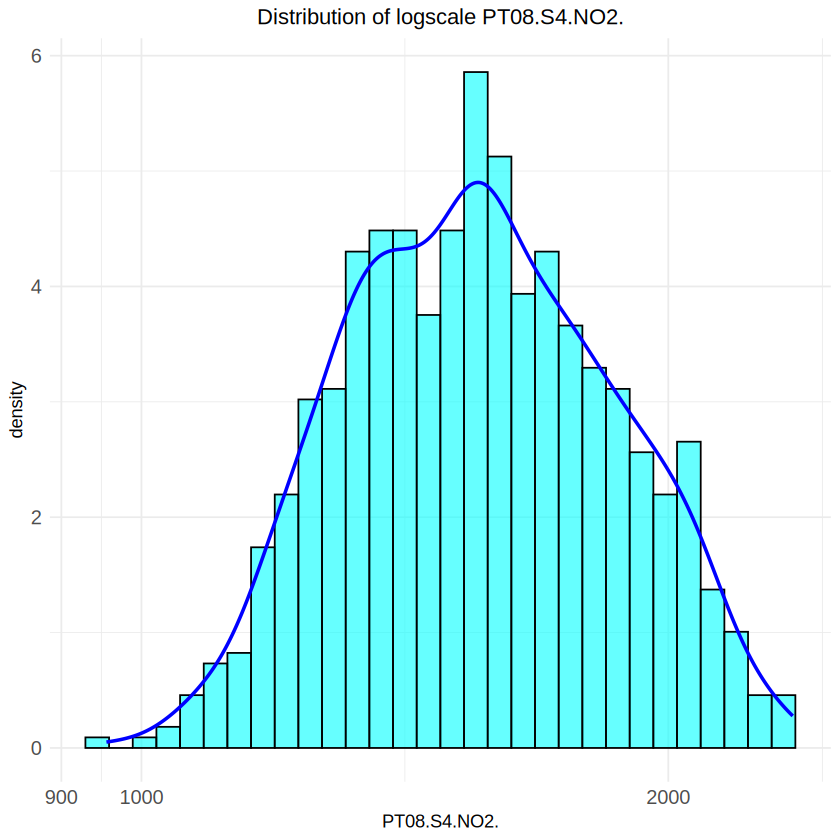
\includegraphics[width=0.75\columnwidth]{air_figures/PT08.S4(NO2)_logscale_distribution.png}
    \caption{Phân phối sau khi log-scale của Sensor response cho Nitrogen oxides.}
    \label{fig:ptno2_logscale_distribution}
\end{figure}
Nhận xét:
\begin{itemize}
    \item Sau khi logscale, ta vẫn thấy phân phối của biến này vẫn xấp xỉ chuẩn
\end{itemize}

\begin{figure}[H]
    \centering
    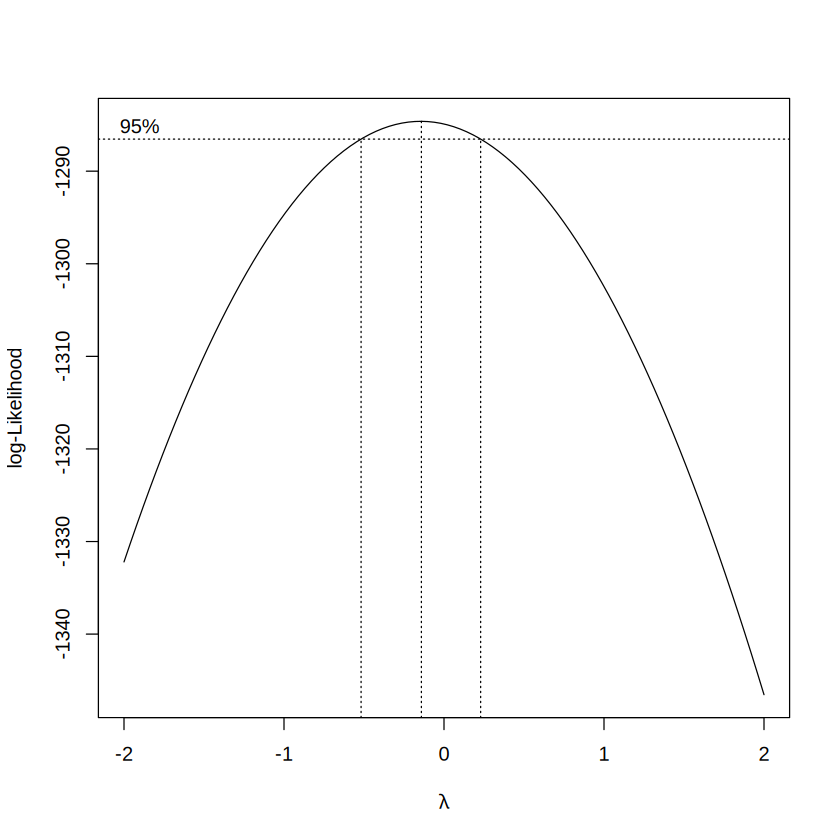
\includegraphics[width=0.75\columnwidth]{air_figures/PT08.S4(NO2)_optimal_lambda.png}
    \caption{Log-likelihood với các giá trị $\lambda$ của Sensor response cho Nitrogen oxides.}
    \label{fig:ptno2_optimal_lambda}
\end{figure}
Nhận xét:
\begin{itemize}
    \item Với mức ý nghĩa 5\%, ta tìm được giá trị lambda phù hợp là 0.7070707
\end{itemize}

Và ta thực hiện biến đổi dữ liệu với giá trị lambda vừa tìm được.
\begin{figure}[H]
    \centering
    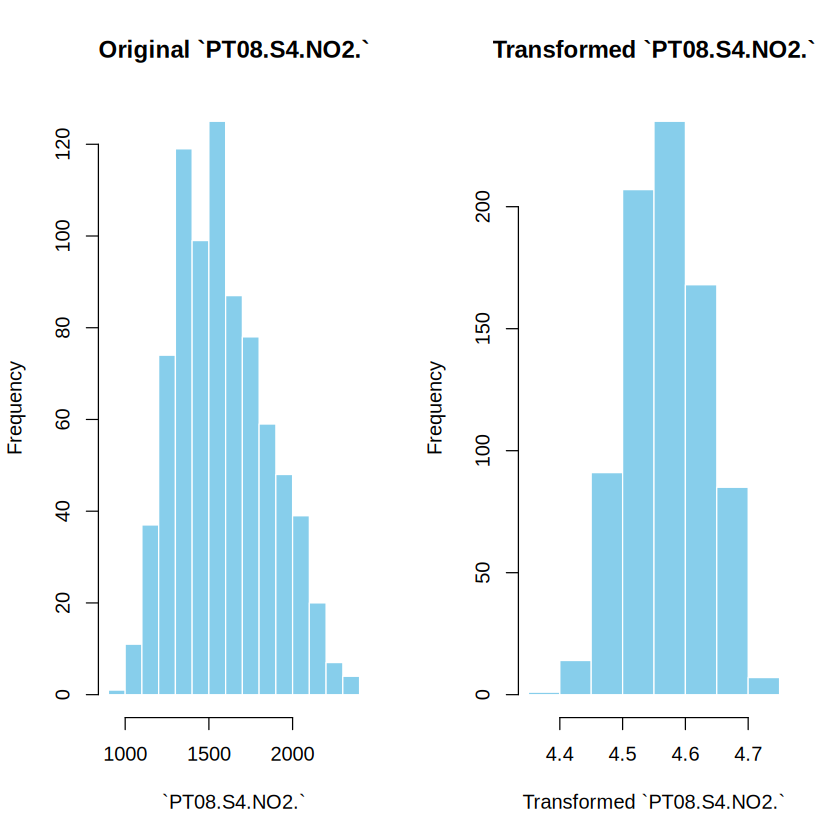
\includegraphics[width=0.75\columnwidth]{air_figures/PT08.S4(NO2)_transformed_distribution.png}
    \caption{Phân phối trước và sau khi biến đổi của Sensor response cho Nitrogen oxides.}
    \label{fig:ptno2_transformed_distribution}
\end{figure}
Nhận xét:
\begin{itemize}
    \item Ta có được giá trị lambda tối ưu là 0.7070707 và sử dụng giá trị này để biến đổi biến PT08.S4(NO2). Biểu đồ histogram phía bên dưới thể hiện phân phối của biến này trước và sau khi biến đổi. Dễ dàng thấy được, sau khi biến đổi, biến này đã tương đối chuẩn hơn.
\end{itemize}

\subsubsection{PT08.S5(O3): Sensor response for ozone}

\begin{figure}[H]
    \centering
    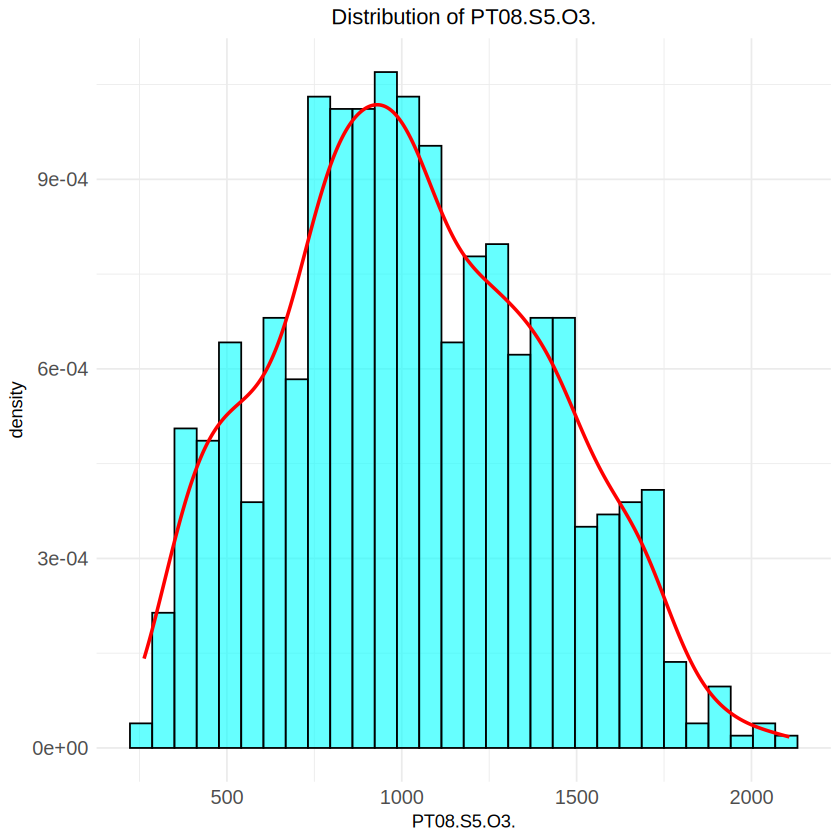
\includegraphics[width=0.75\columnwidth]{air_figures/PT08.S5(O3)_original_distribution.png}
    \caption{Phân phối ban đầu của Sensor response cho Nitrogen oxides.}
    \label{fig:pto3_original_distribution}
\end{figure}

Nhận xét:
\begin{itemize}
    \item Nhìn vào histogram trên, ta thấy phân phối của biến này bị lệch trái (lệch dương).
\end{itemize}

Ta thử sử dụng log-transform nó.

\begin{figure}[H]
    \centering
    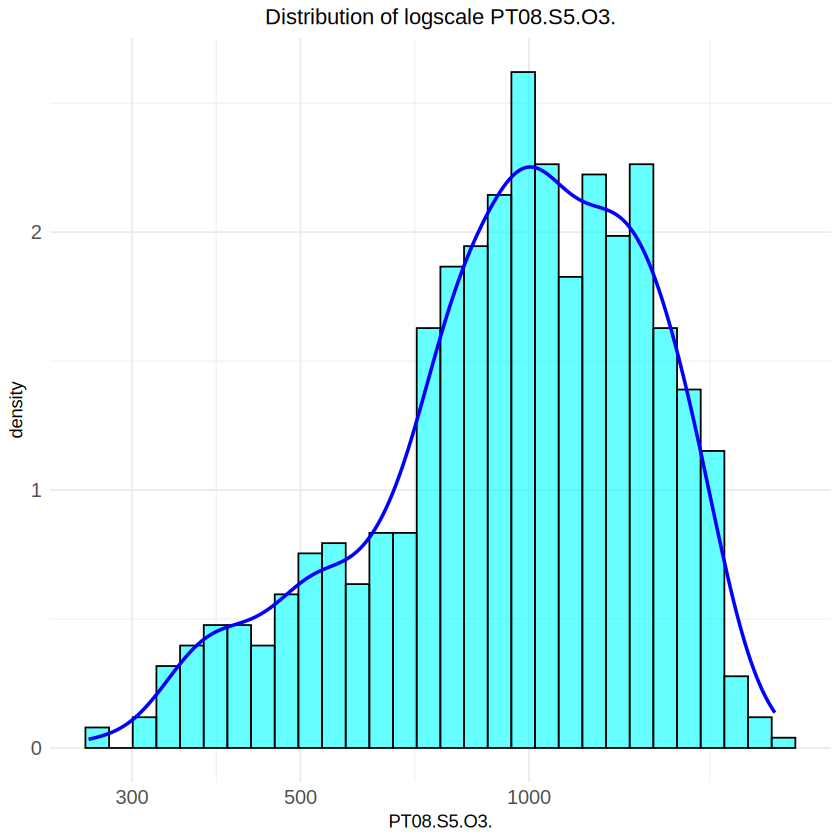
\includegraphics[width=0.75\columnwidth]{air_figures/PT08.S5(O3)_logscale_distribution.png}
    \caption{Phân phối sau khi log-scale của Sensor response cho Nitrogen oxides.}
    \label{fig:pto3_logscale_distribution}
\end{figure}
Nhận xét:
\begin{itemize}
    \item Sau khi logscale, ta thấy phân phối của biến này có chiều hướng lệch phải (lệch âm)
\end{itemize}

\begin{figure}[H]
    \centering
    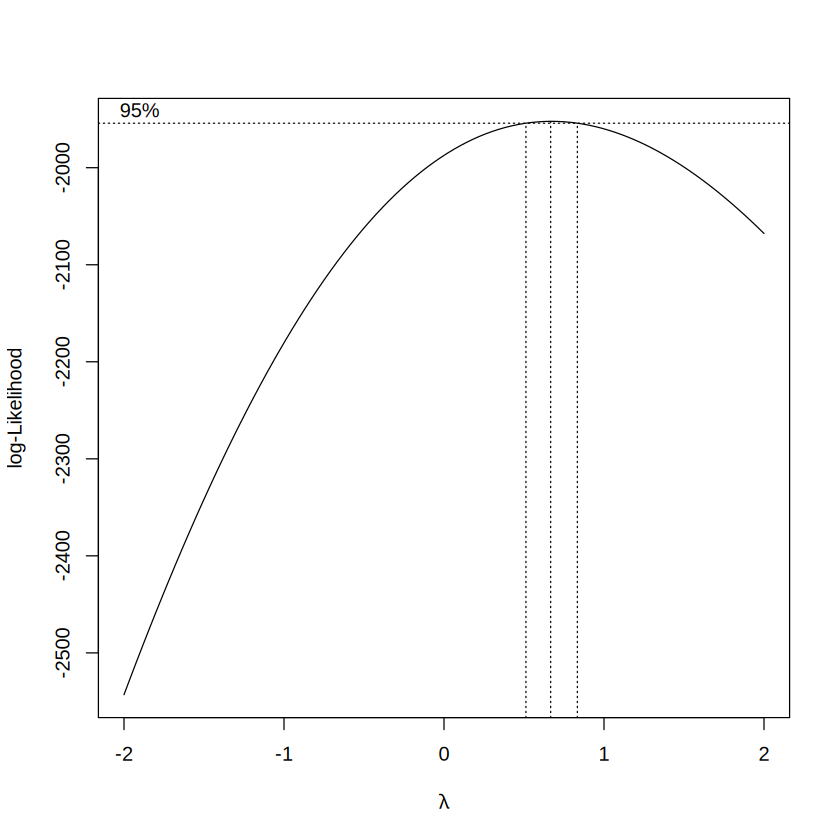
\includegraphics[width=0.75\columnwidth]{air_figures/PT08.S5(O3)_optimal_lambda.png}
    \caption{Log-likelihood với các giá trị $\lambda$ của Sensor response cho Nitrogen oxides.}
    \label{fig:pto3_optimal_lambda}
\end{figure}
Nhận xét:
\begin{itemize}
    \item Với mức ý nghĩa 5\%, ta tìm được giá trị lambda phù hợp 0.3434
\end{itemize}

Và ta thực hiện biến đổi dữ liệu với giá trị lambda vừa tìm được.
\begin{figure}[H]
    \centering
    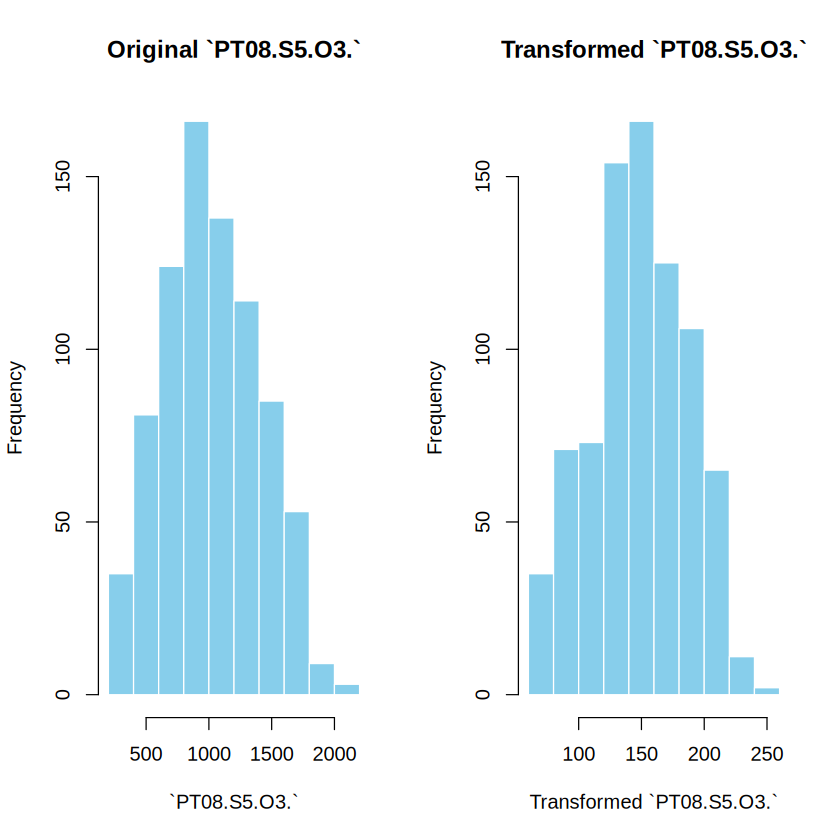
\includegraphics[width=0.75\columnwidth]{air_figures/PT08.S5(O3)_transformed_distribution.png}
    \caption{Phân phối trước và sau khi biến đổi của Sensor response cho Nitrogen oxides.}
    \label{fig:pto3_transformed_distribution}
\end{figure}
Nhận xét:
\begin{itemize}
    \item Ta có được giá trị lambda tối ưu là 0.3434 và sử dụng giá trị này để biến đổi biến PT08.S5(O3). Biểu đồ histogram phía bên dưới thể hiện phân phối của biến này trước và sau khi biến đổi. Dễ dàng thấy được, sau khi biến đổi, biến này đã tương đối chuẩn hơn.
\end{itemize}

\subsubsection{T: Temperature (Celsius)}

\begin{figure}[H]
    \centering
    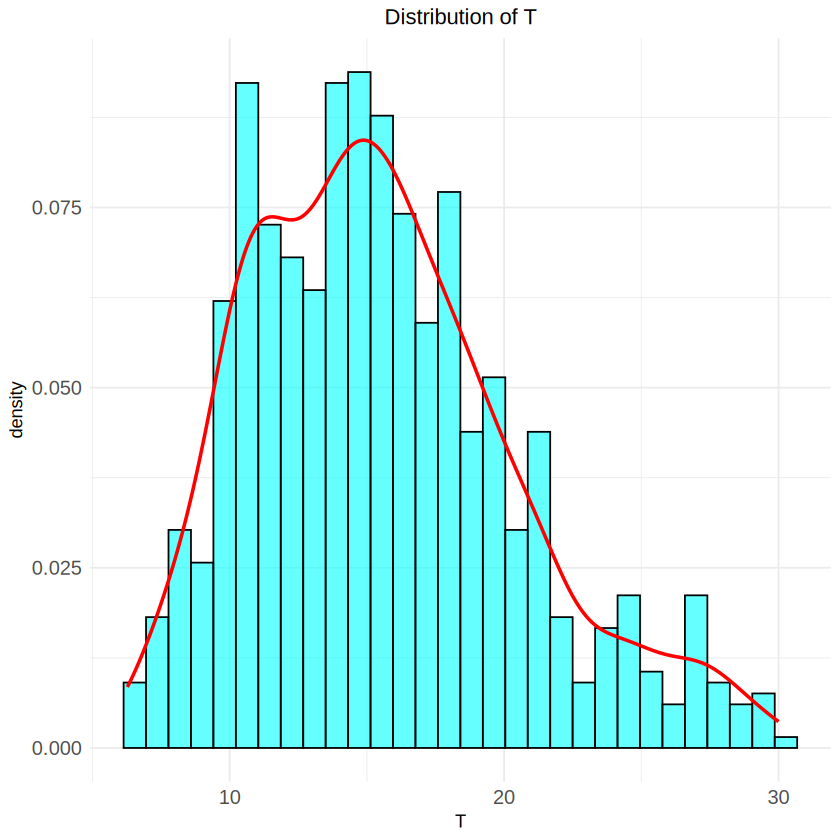
\includegraphics[width=0.75\columnwidth]{air_figures/T_original_distribution.png}
    \caption{Phân phối ban đầu của Sensor response cho Nitrogen oxides.}
    \label{fig:t_original_distribution}
\end{figure}

Nhận xét:
\begin{itemize}
    \item Nhìn vào histogram trên, ta thấy phân phối của biến này bị lệch trái (lệch âm).
\end{itemize}

Ta thử sử dụng log-transform nó.

\begin{figure}[H]
    \centering
    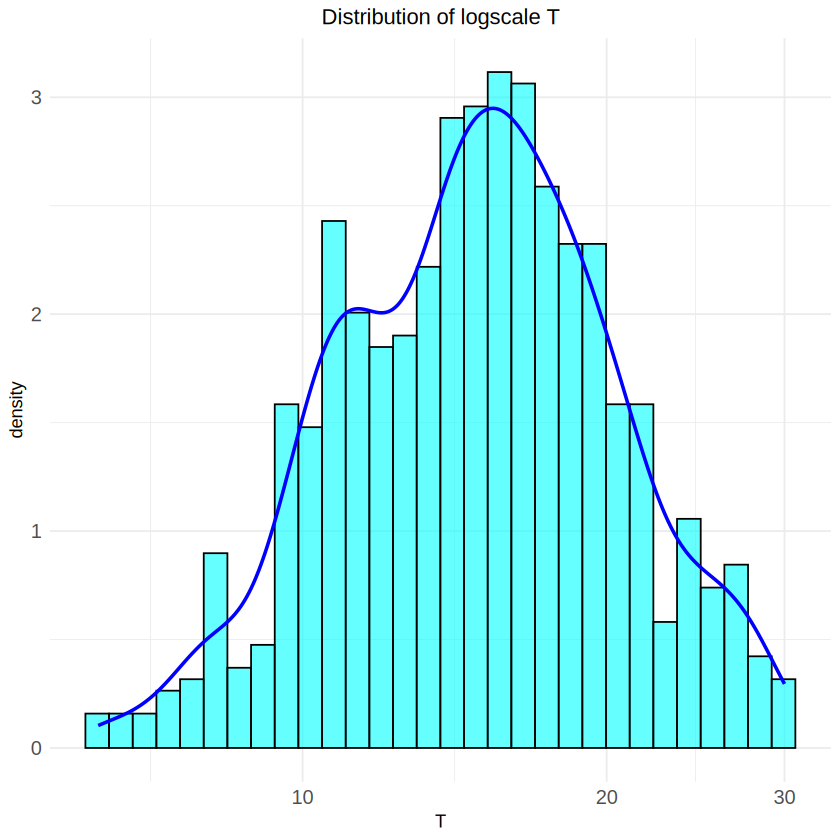
\includegraphics[width=0.75\columnwidth]{air_figures/T_logscale_distribution.png}
    \caption{Phân phối sau khi log-scale của Sensor response cho Nitrogen oxides.}
    \label{fig:t_logscale_distribution}
\end{figure}
Nhận xét:
\begin{itemize}
    \item Sau khi logscale, ta thấy phân phối của biến này có chiều hướng lệch phải (lệch âm)
\end{itemize}

\begin{figure}[H]
    \centering
    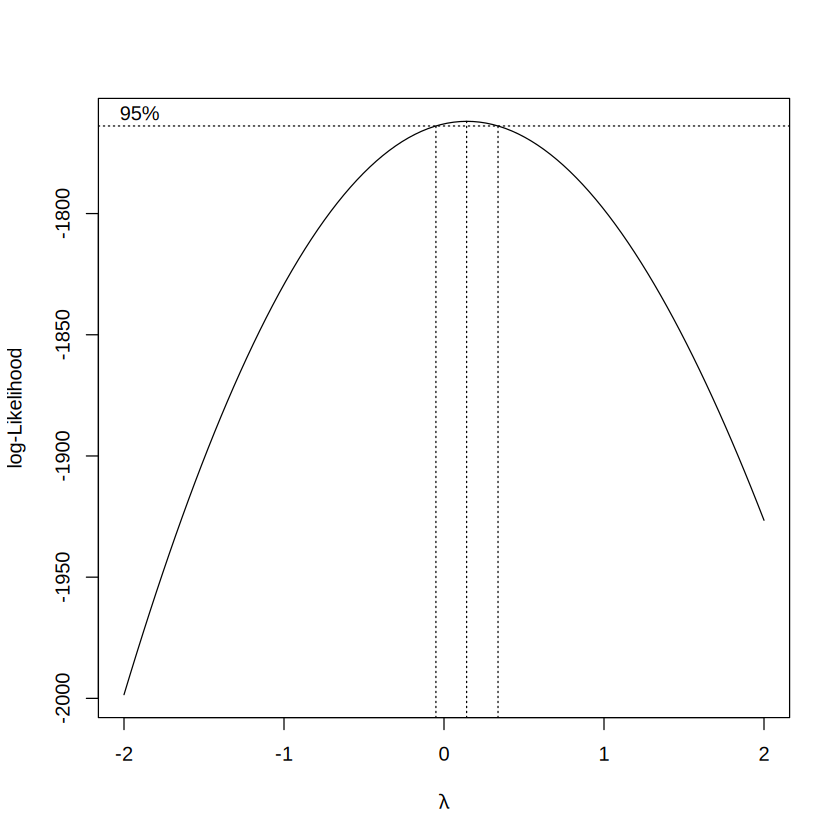
\includegraphics[width=0.75\columnwidth]{air_figures/T_optimal_lambda.png}
    \caption{Log-likelihood với các giá trị $\lambda$ của Sensor response cho Nitrogen oxides.}
    \label{fig:t_optimal_lambda}
\end{figure}
Nhận xét:
\begin{itemize}
    \item Với mức ý nghĩa 5\%, ta tìm được giá trị lambda phù hợp là 0.62626
\end{itemize}

Và ta thực hiện biến đổi dữ liệu với giá trị lambda vừa tìm được.
\begin{figure}[H]
    \centering
    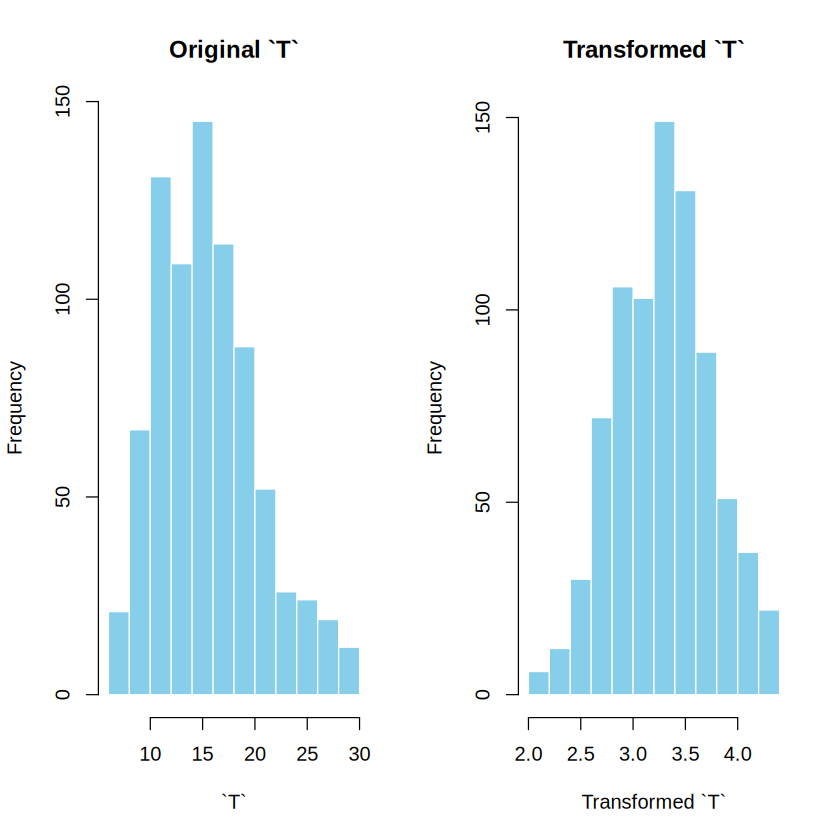
\includegraphics[width=0.75\columnwidth]{air_figures/T_transformed_distribution.png}
    \caption{Phân phối trước và sau khi biến đổi của Sensor response cho Nitrogen oxides.}
    \label{fig:t_transformed_distribution}
\end{figure}
Nhận xét:
\begin{itemize}
    \item Ta có được giá trị lambda tối ưu là 0.62626 và sử dụng giá trị này để biến đổi biến T. Biểu đồ histogram phía bên dưới thể hiện phân phối của biến này trước và sau khi biến đổi. Dễ dàng thấy được, sau khi biến đổi, biến này đã tương đối chuẩn hơn.
\end{itemize}

\subsubsection{RH: Relative humidity (\%)}

\begin{figure}[H]
    \centering
    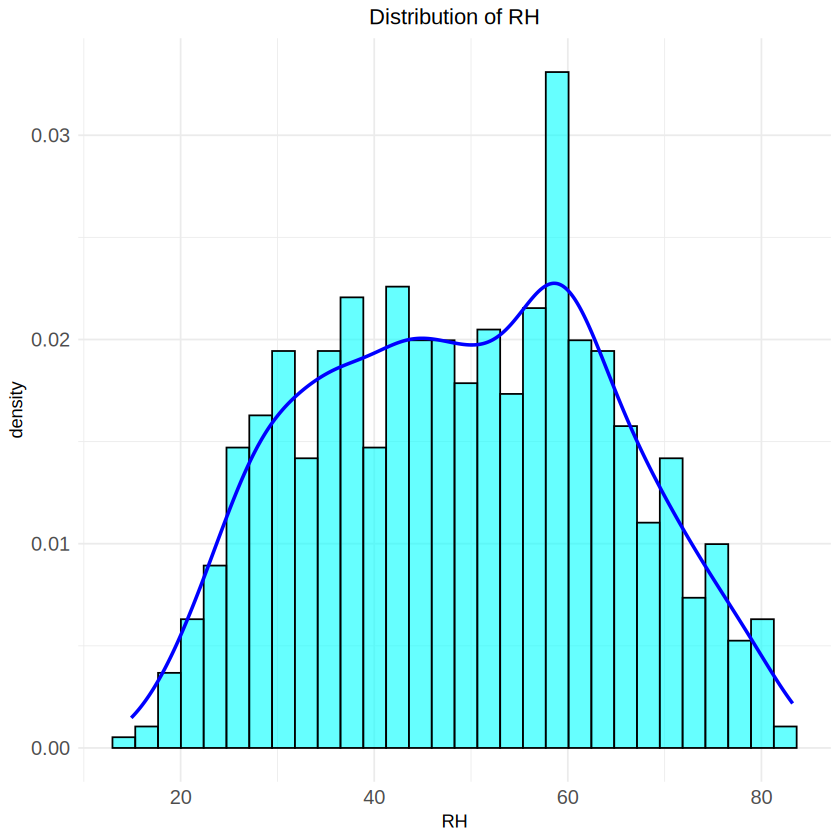
\includegraphics[width=0.75\columnwidth]{air_figures/RH_original_distribution.png}
    \caption{Phân phối ban đầu của Sensor response cho Nitrogen oxides.}
    \label{fig:rh_original_distribution}
\end{figure}

Nhận xét:
\begin{itemize}
    \item Nhìn vào histogram trên, ta thấy phân phối của biến này xấp xỉ chuẩn.
\end{itemize}

Ta thử sử dụng log-transform nó.

\begin{figure}[H]
    \centering
    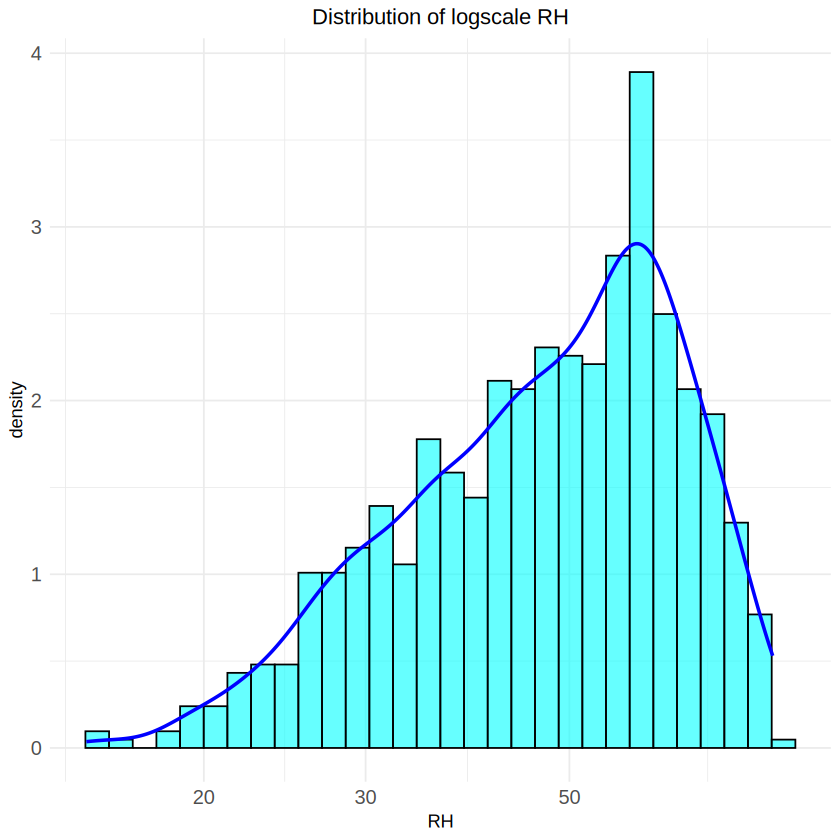
\includegraphics[width=0.75\columnwidth]{air_figures/RH_logscale_distribution.png}
    \caption{Phân phối sau khi log-scale của Sensor response cho Nitrogen oxides.}
    \label{fig:rh_logscale_distribution}
\end{figure}
Nhận xét:
\begin{itemize}
    \item Sau khi logscale, ta thấy phân phối của biến này có chiều hướng lệch phải (lệch âm)
\end{itemize}

\begin{figure}[H]
    \centering
    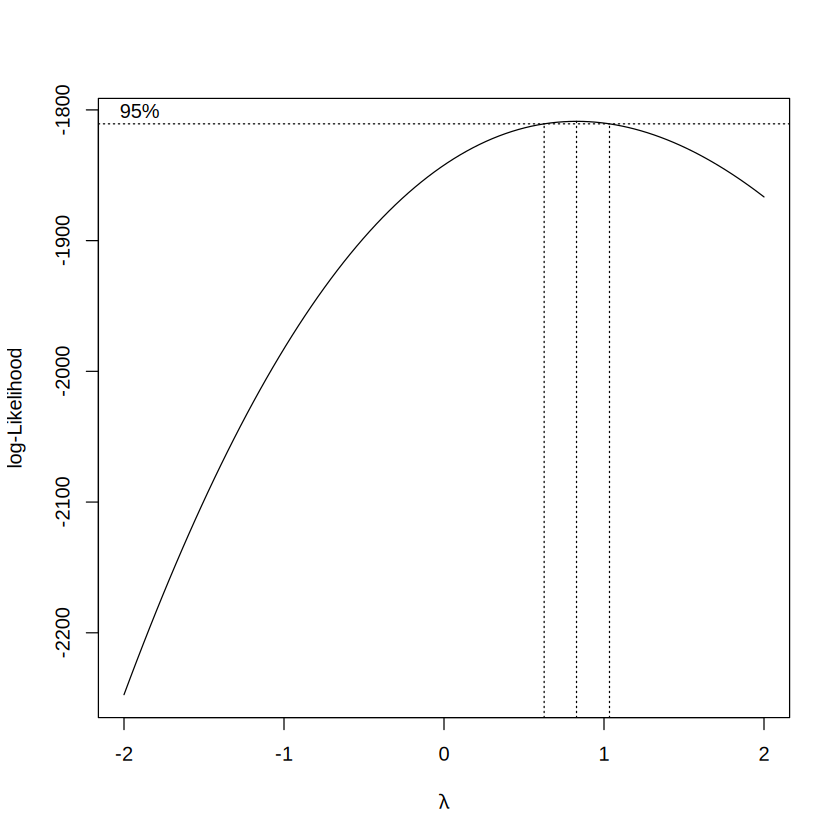
\includegraphics[width=0.75\columnwidth]{air_figures/RH_optimal_lambda.png}
    \caption{Log-likelihood với các giá trị $\lambda$ của Sensor response cho Nitrogen oxides.}
    \label{fig:rh_optimal_lambda}
\end{figure}
Nhận xét:
\begin{itemize}
    \item Với mức ý nghĩa 5\%, ta tìm được giá trị lambda phù hợp 0.909
\end{itemize}

Và ta thực hiện biến đổi dữ liệu với giá trị lambda vừa tìm được.
\begin{figure}[H]
    \centering
    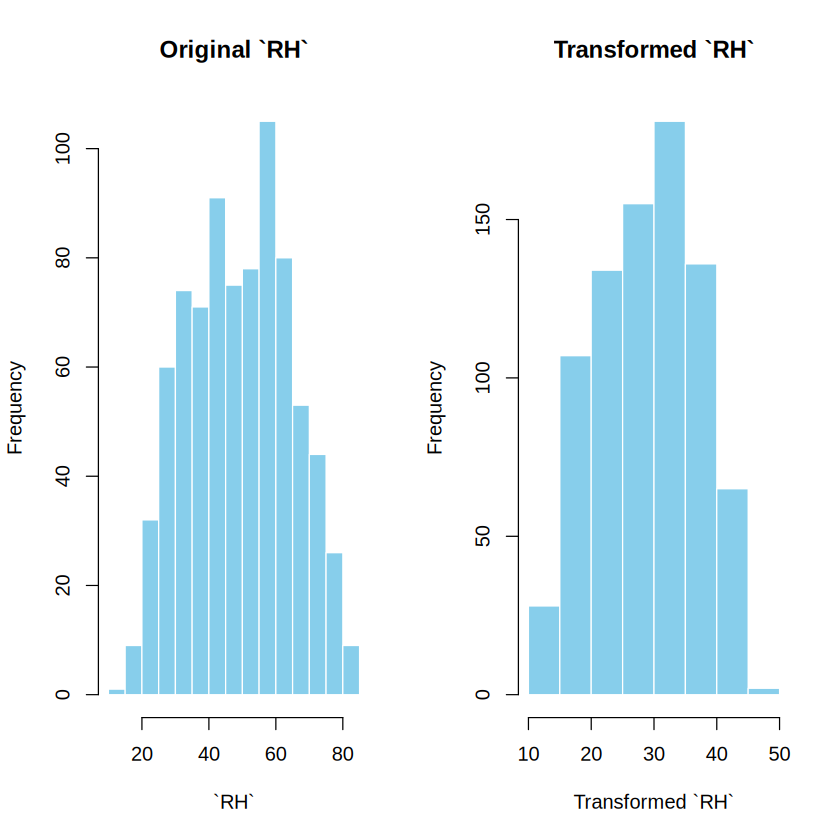
\includegraphics[width=0.75\columnwidth]{air_figures/RH_transformed_distribution.png}
    \caption{Phân phối trước và sau khi biến đổi của Sensor response cho Nitrogen oxides.}
    \label{fig:rh_transformed_distribution}
\end{figure}
Nhận xét:
\begin{itemize}
    \item Ta có được giá trị lambda tối ưu là 0.909 và sử dụng giá trị này để biến đổi biến RH. Biểu đồ histogram phía bên dưới thể hiện phân phối của biến này trước và sau khi biến đổi. Dễ dàng thấy được, sau khi biến đổi, biến này đã tương đối chuẩn hơn.
\end{itemize}

\subsubsection{AH: Absolute humidity ($g/m^3$)}

\begin{figure}[H]
    \centering
    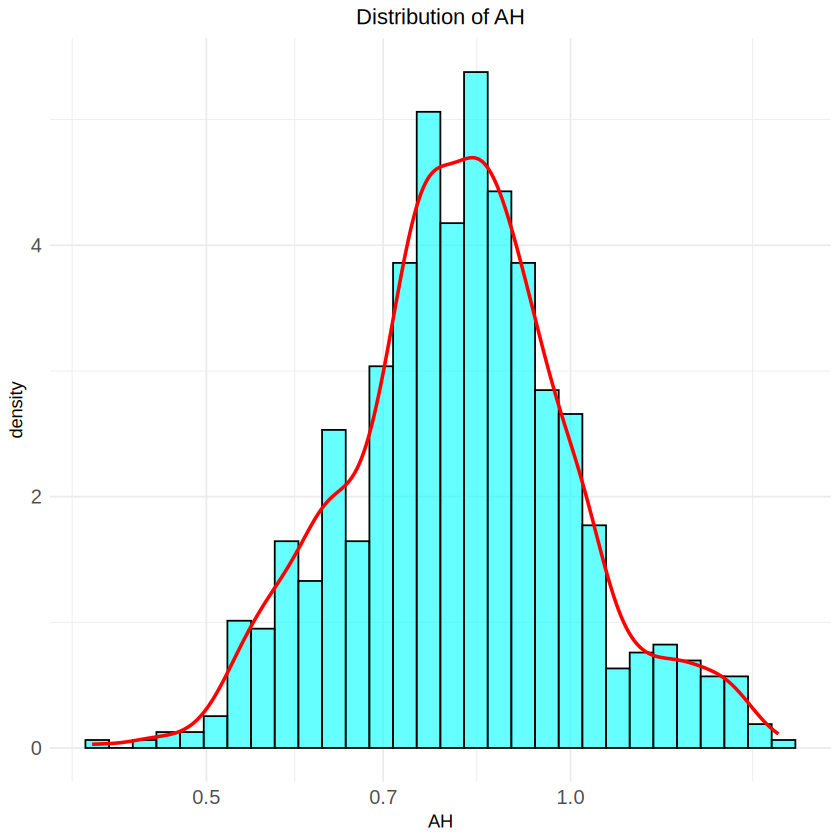
\includegraphics[width=0.75\columnwidth]{air_figures/AH_original_distribution.png}
    \caption{Phân phối ban đầu của Sensor response cho Nitrogen oxides.}
    \label{fig:ah_original_distribution}
\end{figure}

Nhận xét:
\begin{itemize}
    \item Nhìn vào histogram trên, ta thấy phân phối của biến bị lệch phải (lệch âm).
\end{itemize}

Ta thử sử dụng log-transform nó.

\begin{figure}[H]
    \centering
    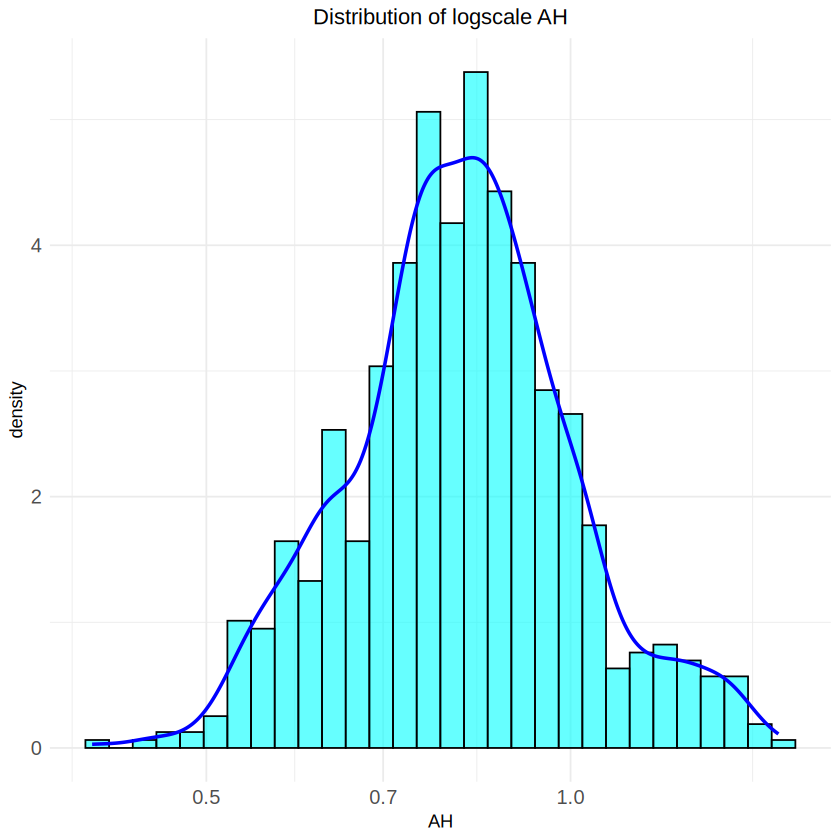
\includegraphics[width=0.75\columnwidth]{air_figures/AH_logscale_distribution.png}
    \caption{Phân phối sau khi log-scale của Sensor response cho Nitrogen oxides.}
    \label{fig:ah_logscale_distribution}
\end{figure}
Nhận xét:
\begin{itemize}
    \item Sau khi logscale, phân phối của biến này vẫn bị lệch.
\end{itemize}

\begin{figure}[H]
    \centering
    \includegraphics[width=0.75\columnwidth]{air_figures/AH_optimal_lambda.png}
    \caption{Log-likelihood với các giá trị $\lambda$ của Sensor response cho Nitrogen oxides.}
    \label{fig:ah_optimal_lambda}
\end{figure}
Nhận xét:
\begin{itemize}
    \item Với mức ý nghĩa 5\%, ta tìm được giá trị lambda phù hợp 0.6666
\end{itemize}

Và ta thực hiện biến đổi dữ liệu với giá trị lambda vừa tìm được.
\begin{figure}[H]
    \centering
    \includegraphics[width=0.75\columnwidth]{air_figures/AH_transformed_distribution.png}
    \caption{Phân phối trước và sau khi biến đổi của Sensor response cho Nitrogen oxides.}
    \label{fig:ah_transformed_distribution}
\end{figure}
Nhận xét:
\begin{itemize}
    \item Ta có được giá trị lambda tối ưu là 0.6666 và sử dụng giá trị này để biến đổi biến AH. Biểu đồ histogram phía bên dưới thể hiện phân phối của biến này trước và sau khi biến đổi. Dễ dàng thấy được, sau khi biến đổi, biến này đã tương đối chuẩn hơn.
    \item Ta để ý thấy có một số ngoại lệ ở giá trị -0.2.
\end{itemize}

\subsection{Phân tích đa biến}

\begin{figure}[H]
    \centering
    \includegraphics[width=0.75\columnwidth]{air_figures/air_corr.png}
    \caption{Ma trận tương quan giữa các biến trong tập dữ liệu Air.}
    \label{fig:air_corr}
\end{figure}
Nhận xét:
\begin{itemize}
    \item Ta thấy các biến trong tập dữ liệu chất lượng không khí có tương quan mạnh với nhau. Điều này có thể chỉ ra rằng trong tập dữ liệu này có hiện tượng đa cộng tuyến rất cao.
\end{itemize}
 Phân tích cụ thể, ta xem xét các biến có mối tương quan thuận mạnh:
 \begin{lstlisting}
  Var1          Var2      value
1         CO.GT.   PT08.S1.CO.  0.7733943
2         CO.GT.      C6H6.GT.  0.8123923
3         CO.GT. PT08.S2.NMHC.  0.7955864
4         CO.GT.       NOx.GT.  0.7622972
5         CO.GT.   PT08.S5.O3.  0.7590266
6    PT08.S1.CO.      C6H6.GT.  0.8838209
7    PT08.S1.CO. PT08.S2.NMHC.  0.8929724
8    PT08.S1.CO.  PT08.S3.NOx. -0.7719181
9    PT08.S1.CO.   PT08.S5.O3.  0.8993259
10      C6H6.GT. PT08.S2.NMHC.  0.9819620
11      C6H6.GT.  PT08.S3.NOx. -0.7357112
12      C6H6.GT.  PT08.S4.NO2.  0.7657168
13      C6H6.GT.   PT08.S5.O3.  0.8657266
14 PT08.S2.NMHC.  PT08.S3.NOx. -0.7966873
15 PT08.S2.NMHC.  PT08.S4.NO2.  0.7772348
16 PT08.S2.NMHC.   PT08.S5.O3.  0.8805903
17       NOx.GT.       NO2.GT.  0.7631329
18  PT08.S3.NOx.   PT08.S5.O3. -0.7965536
 \end{lstlisting}
 Nhận xét:
 \begin{itemize}
     \item Trong dữ liệu, các biến có sự tương quan mạnh với nhau.
     \item  Ta dễ dàng thấy được, đa số cặp tương quan đều có chỉ số cao hơn 0.7
     \item   Điều này giúp chúng ta định hướng được nên sử dụng các mô hình có khả năng xử lý hiện tượng đa cộng tuyến cao trong dữ liệu.
 \end{itemize}

 Và ta cũng xem xét các cặp biến có mối tương quan nghịch mạnh
 \begin{lstlisting}
          Var1         Var2       value
1         CO.GT. PT08.S3.NOx. -0.61387028
2    PT08.S1.CO. PT08.S3.NOx. -0.77191812
3       NMHC.GT. PT08.S3.NOx. -0.26198519
4       NMHC.GT.           RH -0.05279411
5       C6H6.GT. PT08.S3.NOx. -0.73571121
6       C6H6.GT.           RH -0.06164347
7  PT08.S2.NMHC. PT08.S3.NOx. -0.79668731
8  PT08.S2.NMHC.           RH -0.09035172
9        NOx.GT. PT08.S3.NOx. -0.56325927
10       NOx.GT.            T -0.23565652
11       NOx.GT.           AH -0.12683093
12  PT08.S3.NOx.      NO2.GT. -0.56953458
13  PT08.S3.NOx. PT08.S4.NO2. -0.53846012
14  PT08.S3.NOx.  PT08.S5.O3. -0.79655364
15  PT08.S3.NOx.            T -0.14513301
16  PT08.S3.NOx.           RH -0.05672984
17  PT08.S3.NOx.           AH -0.23202063
18       NO2.GT.            T -0.16531710
19       NO2.GT.           RH -0.08064472
20       NO2.GT.           AH -0.29119971
21  PT08.S4.NO2.           RH -0.03218809
22   PT08.S5.O3.            T -0.02719336
23             T           RH -0.57856879
 \end{lstlisting}
Nhận xét:
\begin{itemize}
    \item Chúng ta cũng rút ra kết luận tương tự.
\end{itemize}

\subsubsection{Khảo sát ngoại lai}

Ta sử dụng IQR để tìm các điểm ngoại lai và cực ngoại lai:
\begin{itemize}
    \item Tổng số ngoại lai: 0
    \item Tổng số cực ngoại lai: 0
\end{itemize}

\subsubsection{Chuẩn hóa và phân chia tập dữ liệu}

Ta sử dụng box-cox tranform và sau đó phân chia tập dữ liệu thành 2 phần: train (70\%) và test (30\%).

\subsection{Mô hình hóa bằng hồi quy tuyến tính đa biến}

Trước tiên, ta xây dựng mô hình đầy đủ như sau

\begin{lstlisting}
full.lm <- lm(`C6H6.GT.` ~ ., data = train)
print(summary(full.lm))
\end{lstlisting}
Kết quả:
\begin{lstlisting}
lm(formula = C6H6.GT. ~ ., data = train)

Residuals:
    Min      1Q  Median      3Q     Max 
-1.3855 -0.1963 -0.0553  0.1558  3.9380 

Coefficients:
                Estimate Std. Error t value Pr(>|t|)    
(Intercept)   -1.423e+01  1.795e-01 -79.253  < 2e-16 ***
CO.GT.         4.689e-02  8.772e-03   5.346 9.32e-08 ***
PT08.S1.CO.   -1.518e-03  4.185e-04  -3.626 0.000290 ***
NMHC.GT.       1.064e-03  2.993e-04   3.556 0.000379 ***
PT08.S2.NMHC.  1.083e-01  5.774e-04 187.655  < 2e-16 ***
NOx.GT.        8.187e-03  2.838e-04  28.845  < 2e-16 ***
PT08.S3.NOx.   1.125e-02  3.328e-04  33.819  < 2e-16 ***
NO2.GT.       -1.848e-02  7.815e-04 -23.649  < 2e-16 ***
PT08.S4.NO2.   5.558e-03  3.845e-04  14.453  < 2e-16 ***
PT08.S5.O3.    1.357e-03  2.494e-04   5.443 5.44e-08 ***
T             -8.847e-02  7.468e-03 -11.846  < 2e-16 ***
RH            -4.064e-02  3.545e-03 -11.464  < 2e-16 ***
AH             5.389e-01  4.896e-02  11.008  < 2e-16 ***
---
Signif. codes:  0 '***' 0.001 '**' 0.01 '*' 0.05 '.' 0.1 ' ' 1
...
Residual standard error: 0.3119 on 6536 degrees of freedom
Multiple R-squared:  0.9923,	Adjusted R-squared:  0.9923 
F-statistic: 7.05e+04 on 12 and 6536 DF,  p-value: < 2.2e-16
\end{lstlisting}
Nhận xét:
\begin{itemize}
    \item Mô hình có R-squared là 0.9923, tức là 99.23\% phương sai của biến C6H6.GT. được giải thích bởi các biến độc lập trong mô hình.
\end{itemize}

Tiếp theo, ta định nghĩa mô hình chặn trên và chặn dưới để lựa chọn mô hình
\begin{lstlisting}
# Mô hình chặn dưới
model.lb <- lm(`C6H6.GT.` ~ 1, data = train) 

# Mô hình chặn trên
model.up <- full.lm

step(full.lm, scope = list(lower = model.lb, upper = model.up), direction = "both", trace = FALSE)
\end{lstlisting}
Kết quả:
\begin{lstlisting}
lm(formula = C6H6.GT. ~ CO.GT. + PT08.S1.CO. + NMHC.GT. + PT08.S2.NMHC. + 
    NOx.GT. + PT08.S3.NOx. + NO2.GT. + PT08.S4.NO2. + PT08.S5.O3. + 
    T + RH + AH, data = train)

Coefficients:
  (Intercept)         CO.GT.    PT08.S1.CO.       NMHC.GT.  PT08.S2.NMHC.  
   -14.229708       0.046891      -0.001518       0.001064       0.108347  
      NOx.GT.   PT08.S3.NOx.        NO2.GT.   PT08.S4.NO2.    PT08.S5.O3.  
     0.008187       0.011255      -0.018483       0.005558       0.001357  
            T             RH             AH  
    -0.088472      -0.040642       0.538945  
\end{lstlisting}

\begin{lstlisting}
air_models<- regsubsets(C6H6.GT. ~ CO.GT. + PT08.S1.CO. + NMHC.GT. + PT08.S2.NMHC. + 
    NOx.GT. + PT08.S3.NOx. + NO2.GT. + PT08.S4.NO2. + PT08.S5.O3. + 
    T + RH + AH, data = train)
summary.air<-summary(air_models)

# Lựa chọn mô hình tốt nhất từ reg subsets 
summary.air$which
\end{lstlisting}
Ta lựa chọn mô hình tốt nhất dựa trên BIC
\begin{lstlisting}
# Tiêu chí chọn mô hình tốt nhất 4: mô hình với BIC nhỏ
summary.air$bic

best_model_index <- which.min(summary.csm$bic)
best_model <- summary.csm$which[best_model_index, ]
print(best_model)
best_vars <- names(best_model[best_model])
best_vars <- best_vars[best_vars != "(Intercept)"]
print(best_vars)
\end{lstlisting}
Kết quả:
\begin{lstlisting}
(Intercept)        CO.GT.   PT08.S1.CO.      NMHC.GT. PT08.S2.NMHC. 
         TRUE         FALSE         FALSE         FALSE          TRUE 
      NOx.GT.  PT08.S3.NOx.       NO2.GT.  PT08.S4.NO2.   PT08.S5.O3. 
         TRUE          TRUE          TRUE          TRUE         FALSE 
            T            RH            AH 
         TRUE          TRUE          TRUE 
[1] "PT08.S2.NMHC." "NOx.GT."       "PT08.S3.NOx."  "NO2.GT."      
[5] "PT08.S4.NO2."  "T"             "RH"            "AH"           
\end{lstlisting}

Xây dựng mô hình tốt nhất
\begin{lstlisting}
# Xây dựng mô hình tốt nhất
formula_str <- paste("C6H6.GT. ~", paste(best_vars, collapse = " + "))
best_model_air <- lm(as.formula(formula_str), data=train)

# Tóm tắt mô hình
summary(best_model_air)
\end{lstlisting}
Kết quả:
\begin{lstlisting}
lm(formula = as.formula(formula_str), data = train)

Residuals:
    Min      1Q  Median      3Q     Max 
-1.3449 -0.1997 -0.0546  0.1609  3.8753 

Coefficients:
                Estimate Std. Error t value Pr(>|t|)    
(Intercept)   -1.434e+01  1.717e-01  -83.53   <2e-16 ***
PT08.S2.NMHC.  1.091e-01  5.156e-04  211.67   <2e-16 ***
NOx.GT.        8.707e-03  2.648e-04   32.88   <2e-16 ***
PT08.S3.NOx.   1.081e-02  3.248e-04   33.27   <2e-16 ***
NO2.GT.       -1.743e-02  7.717e-04  -22.59   <2e-16 ***
PT08.S4.NO2.   5.917e-03  3.628e-04   16.31   <2e-16 ***
T             -9.191e-02  7.381e-03  -12.45   <2e-16 ***
RH            -4.096e-02  3.558e-03  -11.51   <2e-16 ***
AH             5.359e-01  4.887e-02   10.97   <2e-16 ***
---
Signif. codes:  0 '***' 0.001 '**' 0.01 '*' 0.05 '.' 0.1 ' ' 1

Residual standard error: 0.3136 on 6540 degrees of freedom
Multiple R-squared:  0.9922,	Adjusted R-squared:  0.9922 
F-statistic: 1.046e+05 on 8 and 6540 DF,  p-value: < 2.2e-16
\end{lstlisting}
Nhận xét:
\begin{itemize}
    \item Mô hình có R-squared là 0.9922, tức là 99.22\% phương sai của biến C6H6.GT. được giải thích bởi các biến độc lập trong mô hình.
\end{itemize}

Bây giờ, ta sẽ đi phân tích mô hình này. 
\begin{figure}[H]
    \centering
    \includegraphics[width=0.75\columnwidth]{air_figures/best_model_air.png}
    \caption{.}
    \label{fig:best_model_air}
\end{figure}

\textbf{Phân tích Residuals vs Fitted Plot}: Biểu đồ Residuals vs Fitted Plot đưa ra dấu hiệu nếu có các mẫu phi tuyến tính. Để hồi quy tuyến tính chính xác, dữ liệu cần phải tuyến tính nên điều này sẽ kiểm tra xem điều kiện đó có được đáp ứng hay không.

\begin{figure}[H]
    \centering
    \includegraphics[width=0.75\columnwidth]{air_figures/best_model_air_residual_fitted.png}
    \caption{Biểu đồ Residuals vs Fitted Plot của mô hình hồi quy Air.}
    \label{fig:best_model_air_residual_fitted}
\end{figure}
Nhận xét:
\begin{itemize}
    \item Dựa trên biểu đồ này, ta thấy đường cong màu đỏ có dáng gần như một đường thẳng, và các phần tử trải dọc theo đường cong này một cách tương đồng đều. Điều này chứng tỏ không có quan hệ phi tuyến xuất hiện trong dữ liệu.
\end{itemize}


\textbf{Phân tích Normal Q–Q (quantile-quantile) Plot}: Các giá trị thặng dư (residual) nên có phân phối chuẩn. Để kiểm tra điều này, chúng ta cần quan sát biểu đồ QQ Residuals plot, nếu các điểm được xếp thành một đường thẳng (hoặc gần như thẳng) thì chứng tỏ các giá trị thặng dư (residual) có phân phối chuẩn.
\begin{figure}[H]
    \centering
    \includegraphics[width=0.75\columnwidth]{air_figures/best_model_air_qq.png}
    \caption{Normal Q–Q (quantile-quantile) Plot cho mô hình hồi quy Air.}
    \label{fig:best_model_air_qq}
\end{figure}

Cẩn thận hơn, chúng ta thử dùng Shapiro–Wilk test để kiểm tra có đúng thật là các giá trị thặng dư có phân phối chuẩn hay không?
\begin{itemize}
    \item H0: Biến thặng dư của mô hình phân phối chuẩn trong một số quần thể.
    \item H1: Biến thặng dư của mô hình không phân phối chuẩn trong một số quần thể.
\end{itemize}

Kết quả:
\begin{lstlisting}
Shapiro-Wilk normality test

data:  model$residuals[3:5000]
W = 0.96092, p-value < 2.2e-16

[1] "H0 rejected: the residuals are NOT distributed normally"
\end{lstlisting}

Kết quả cho thấy p-value bé hơn mức ý nghĩa alpha 0.05 nên ta có thể bác bỏ giả thhuyết H0, biến thặng dư của chúng ta không chuẩn trong một số quần thể. Do biến thặng dư không thoả mãn được tính chuẩn nên những phân tích về sau có thể không đảm bảo độ tin cậy.

\begin{figure}[H]
    \centering
    \includegraphics[width=0.75\columnwidth]{air_figures/best_model_air_histogram_residual.png}
    \caption{Histogram biến thặng dư của mô hình hồi quy Air.}
    \label{fig:best_model_air_histogram_residual}
\end{figure}

\textbf{Phân tích Scale-Location}: Biểu đồ scale-location kiểm định giả định hồi quy về phương sai bằng nhau (homoscedasticity), tức là giá trị thặng dư có phương sai bằng với đường hồi quy.

\begin{figure}[H]
    \centering
    \includegraphics[width=0.75\columnwidth]{air_figures/best_model_air_scale.png}
    \caption{Scale-Location Plot cho mô hình hồi quy Air.}
    \label{fig:best_model_air_scale}
\end{figure}
Nhận xét:
\begin{itemize}
    \item Đường màu đỏ gần bị lệch về phía dưới của biểu đồ. Nghĩa là, độ phân tán của giá trị thặng dư gần không bằng nhau ở tất cả các giá trị phù hợp. 
    \item  Các giá trị thặng dư được phân tán ngẫu nhiên xung quanh đường màu đỏ với độ biến thiên tương đối bằng nhau ở tất cả các giá trị phù hợp.
\end{itemize}

Cẩn thận hơn, chúng ta sử dụng Breusch-Pagan test để kiểm tra có thật là như vậy không?
\begin{itemize}
    \item H0: Các giá trị thặng dư là homoscedastic
    \item H1: Các giá trị thặng dư là heteroscedastic
\end{itemize}
Kết quả:
\begin{lstlisting}
studentized Breusch-Pagan test

data:  model
BP = 1157, df = 8, p-value < 2.2e-16

[1] "H0 rejected: Error variance spreads INCONSTANTLY/generating patterns (Heteroscedasticity)"
\end{lstlisting}
Như vậy, ta thấy p-value lớn hơn múc ý nghĩa 0.05, ta đủ điều kiện bác bỏ H0. Vậy các giá trị thặng dư là heteroscedasticity.

\textbf{Phân tích Residuals vs Leverage} Biểu đồ này có thể được sử dụng để tìm các trường hợp có ảnh hưởng trong tập dữ liệu. Một trường hợp có ảnh hưởng là một trường hợp mà nếu bị loại bỏ sẽ ảnh hưởng đến mô hình nên việc đưa vào hoặc loại trừ nó cần được xem xét.

Một trường hợp có ảnh hưởng có thể là một trường hợp ngoại lệ hoặc không và mục đích của biểu đồ này là xác định các trường hợp có ảnh hưởng lớn đến mô hình. Các ngoại lệ sẽ có xu hướng có giá trị cực cao hoặc cực thấp và do đó ảnh hưởng đến mô hình.

\begin{figure}[H]
    \centering
    \includegraphics[width=0.75\columnwidth]{air_figures/best_model_air_residual_leverage.png}
    \caption{Residuals vs Leverage Plot cho mô hình hồi quy Air.}
    \label{fig:best_model_air_residual_leverage}
\end{figure}
Nhận xét:
\begin{itemize}
    \item Một số điểm như 1840, 6101, 6100 có thể là các điểm ngoại lai. Ta có thể thử loại bỏ để nâng cao chất lượng mô hình.
\end{itemize}

Ta cũng có thể nhận thấy có một số giá trị ngoại lai ở cách xa đường thằng giữa. Ta có thể xem rõ hơn thông qua histogram của Cook's Distance
\begin{figure}[H]
    \centering
    \includegraphics[width=0.75\columnwidth]{air_figures/best_model_air_cook.png}
    \caption{Cook Distance Plot của mô hình hồi quy CSM.}
    \label{fig:best_model_air_cook}
\end{figure}

Bằng cách loại bỏ các điểm ảnh hưởng dựa trên Cook Distance, ta thử nghiệm việc loại bỏ các giá trị này để xem liệu mô hình có thỏa mãn các điều kiện của mô hình hồi quy tuyến tính hay không. Tuy nhiên, các lần thử nghiệm cho đều cho thấy phân phối của biến thặng dư không chuẩn. Do đó, các phân tích về sau có thể không đảm bảo được tính tin cậy.

Ta trực quan kết quả dự đoán và đánh giá RMSE của mô hình đã chọn.

\begin{figure}[H]
    \centering
    \includegraphics[width=0.75\columnwidth]{air_figures/best_model_air_prediction.png}
    \caption{Trực quan kết quả dự đoán của mô hình Air tốt nhất. RMSE = 0.5201.}
    \label{fig:best_model_air_predictiont}
\end{figure}

Hiệu suất trên các độ đo:
\begin{itemize}
    \item R-squared: 0.974160108813221
    \item RMSE:  0.520176239781131
\end{itemize}


\subsection{Mô hình hóa bằng PCR}

Principal Component Regression (PCR) là một kỹ thuật kết hợp Phân tích thành phần chính (PCA) và hồi quy tuyến tính để giải quyết đa cộng tuyến và giảm chiều trong các tập dữ liệu cao chiều. Các bước chính trong PCR là:
\begin{itemize}
    \item PCA biến đổi các biến dự báo ban đầu thành một tập hợp các biến mới, không tương quan được gọi là các thành phần chính. Các thành phần này là các tổ hợp tuyến tính của các biến ban đầu và được sắp xếp theo lượng phương sai mà chúng giải thích trong dữ liệu. Mỗi thành phần chính nắm bắt được phương sai tối đa có thể trong khi vẫn trực giao với các thành phần trước đó.
    \item Một tập hợp con các thành phần chính (giải thích phương sai lớn nhất) được chọn và sử dụng làm các yếu tố dự báo trong mô hình hồi quy tuyến tính để dự báo biến phản hồi. Bằng cách tập trung vào các thành phần chính nắm bắt được phương sai lớn nhất, PCR hướng đến mục tiêu xây dựng một mô hình hồi quy ổn định và dễ diễn giải hơn.
\end{itemize}

\begin{lstlisting}
# Fitting the PCR model on the training data
pcr_model <- pcr(`C6H6.GT.` ~ ., data = train, scale = TRUE, validation = "CV") # Fit PCR model with cross-validation

summary(pcr_model)
\end{lstlisting}

Đối số xác thực = “CV” chỉ định rằng xác thực chéo (cross-validation - CV) nên được sử dụng để xác thực mô hình. Xác thực chéo là một phương pháp mạnh mẽ để đánh giá hiệu suất dự đoán của một mô hình. Nó bao gồm việc phân vùng dữ liệu thành các tập hợp con, huấn luyện mô hình trên một số tập hợp con (bộ huấn luyện - training set) và xác thực nó trên các tập hợp con còn lại (bộ xác thực - validation set). Quá trình này được lặp lại nhiều lần để đảm bảo hiệu suất của mô hình là nhất quán và không phụ thuộc vào phân vùng dữ liệu cụ thể.

Bằng cách sử dụng xác thực chéo, mô hình ít có khả năng quá khớp với dữ liệu huấn luyện. Quá khớp xảy ra khi mô hình nắm bắt được nhiễu và các mẫu cụ thể trong dữ liệu huấn luyện không tổng quát hóa thành dữ liệu mới, chưa từng thấy. Xác thực chéo giúp phát hiện và giảm thiểu tình trạng quá khớp bằng cách kiểm tra mô hình trên các tập hợp con khác nhau của dữ liệu.

Và ta có kết quả như sau:
\begin{lstlisting}
Data: 	X dimension: 6549 12 
	Y dimension: 6549 1
Fit method: svdpc
Number of components considered: 12

VALIDATION: RMSEP
Cross-validated using 10 random segments.
       (Intercept)  1 comps  2 comps  3 comps  4 comps  5 comps  6 comps
CV           3.559    1.063    1.053    1.016    1.001   0.7721   0.7637
adjCV        3.559    1.063    1.053    1.016    1.001   0.7721   0.7637
       7 comps  8 comps  9 comps  10 comps  11 comps  12 comps
CV      0.7315   0.7142   0.5740    0.5741    0.3266    0.3129
adjCV   0.7314   0.7141   0.5738    0.5740    0.3265    0.3128

TRAINING: % variance explained
          1 comps  2 comps  3 comps  4 comps  5 comps  6 comps  7 comps
X           51.80    68.66    80.52    87.53    92.94    95.34    97.08
C6H6.GT.    91.09    91.26    91.86    92.10    95.30    95.41    95.79
          8 comps  9 comps  10 comps  11 comps  12 comps
X           98.14    98.95     99.65     99.89    100.00
C6H6.GT.    95.99    97.41     97.41     99.17     99.23
\end{lstlisting}

\textbf{Lựa chọn số lượng thành phần chính}: Để quyết định được số thành phần chính tối ưu, chúng ta cần phải trung hòa giữa độ phức tạp của mô hình (tức là số lượng components) và RMSEP (Root Mean Squared Error of Prediction).

\begin{figure}[H]
    \centering
    \includegraphics[width=0.75\columnwidth]{air_figures/pcr_model.png}
    \caption{Giá trị RMSEP với số lượng thành phần chính khác nhau của mô hình Air PCR.}
    \label{fig:air_pcr_model}
\end{figure}
Nhận xét:
\begin{itemize}
    \item Dựa trên RMSEP, ta thấy khi sử dụng 12 component mô hình cho kết quả RMSE thấp nhất. Do đó, ta sẽ chọn 12 components
\end{itemize}

\begin{lstlisting}
# Predict using the model and evaluate on the test set with optimal number of components
optimal_number_of_components <- 12  # Optimal number of components based on the RMSEP plot and summary
predictions <- predict(pcr_model, ncomp = optimal_number_of_components, newdata = test)  

# Compare predictions with actual values
plot(test$`C6H6.GT.`, predictions, xlab = "Actual", ylab = "Predicted", main = "Predicted vs Actual C6H6(GT) Values (PCR Model)")  # Plot actual vs predicted values
abline(0, 1)  # Add a diagonal line for reference
\end{lstlisting}

\textbf{Đánh giá kết quả dự đoán}
\begin{figure}[H]
    \centering
    \includegraphics[width=0.75\columnwidth]{air_figures/pcr_prediction.png}
    \caption{Kết quả dự đoán của mô hình Air PCR.}
    \label{fig:air_pcr_prediction}
\end{figure}

Tính toán RMSE
\begin{lstlisting}
# Calculate and print the Root Mean Squared Error (RMSE)
rmse <- sqrt(mean((test$`C6H6.GT.` - predictions)^2))  # Calculate RMSE between actual and predicted values
print(paste("RMSE: ", rmse)) 
\end{lstlisting}
Kết quả: RMSE = 0.517225894818149

Tính toán R-squared
\begin{lstlisting}
# Calculate the sum of squares of residuals
ss_res <- sum((test$`C6H6.GT.` - predictions)^2)

# Calculate the total sum of squares
ss_tot <- sum((test$`C6H6.GT.` - mean(test$`C6H6.GT.`))^2)

# Calculate R-squared
r_squared <- 1 - (ss_res / ss_tot)

# Print R-squared
print(paste("R-squared: ", r_squared))
\end{lstlisting}

Kết quả: R-squared = 0.97445239587654

\subsection{Mô hình hóa bằng PLS}

Partial Least Squares Regression là một kỹ thuật, không giống như PCR, xem xét cả các biến dự báo và biến phản hồi trong quá trình giảm chiều. Các bước chính trong PLS là:
\begin{itemize}
    \item Latent Variable Extraction: PLS trích xuất một tập hợp các biến tiềm ẩn (thành phần) tối đa hóa hiệp phương sai giữa các biến dự báo và biến phản hồi. Các thành phần này là các tổ hợp tuyến tính của các biến ban đầu, được chọn theo cách mà chúng nắm bắt được càng nhiều thông tin có liên quan càng tốt để dự đoán biến phản hồi. Điều này đảm bảo rằng các thành phần được trích xuất có liên quan trực tiếp đến kết quả quan tâm.
    \item Regression: Các biến tiềm ẩn sau đó được sử dụng làm biến dự báo trong mô hình hồi quy tuyến tính để dự báo biến phản hồi. Bằng cách kết hợp biến phản hồi vào quy trình trích xuất thành phần, PLS hướng đến mục tiêu cải thiện độ chính xác dự báo của mô hình hồi quy.
\end{itemize}

\begin{lstlisting}
# Fitting the PLS model on the training data
pls_model <- plsr(`C6H6.GT.` ~ ., data = train, scale = TRUE, validation = "CV")

summary(pls_model)
\end{lstlisting}

Và ta có kết quả:
\begin{lstlisting}
Data: 	X dimension: 6549 12 
	Y dimension: 6549 1
Fit method: kernelpls
Number of components considered: 12

VALIDATION: RMSEP
Cross-validated using 10 random segments.
       (Intercept)  1 comps  2 comps  3 comps  4 comps  5 comps  6 comps
CV           3.559   0.9928   0.7452   0.6638   0.6035   0.4785   0.4408
adjCV        3.559   0.9928   0.7450   0.6638   0.6035   0.4783   0.4407
       7 comps  8 comps  9 comps  10 comps  11 comps  12 comps
CV      0.3843   0.3322   0.3156    0.3145     0.313    0.3131
adjCV   0.3842   0.3321   0.3156    0.3144     0.313    0.3130

TRAINING: % variance explained
          1 comps  2 comps  3 comps  4 comps  5 comps  6 comps  7 comps
X           51.76    60.82    72.13    82.96    87.34    92.87    95.43
C6H6.GT.    92.23    95.63    96.54    97.14    98.21    98.48    98.84
          8 comps  9 comps  10 comps  11 comps  12 comps
X           96.64    98.12     99.15     99.30    100.00
C6H6.GT.    99.14    99.22     99.23     99.23     99.23
\end{lstlisting}

\textbf{Lựa chọn số lượng thành phần chính}: Để quyết định được số thành phần chính tối ưu, chúng ta cần phải trung hòa giữa độ phức tạp của mô hình (tức là số lượng components) và RMSEP (Root Mean Squared Error of Prediction).

\begin{figure}[H]
    \centering
    \includegraphics[width=0.75\columnwidth]{air_figures/pls_model.png}
    \caption{Giá trị RMSEP với số lượng thành phần chính khác nhau của mô hình Air PLS.}
    \label{fig:air_pls_model}
\end{figure}
Nhận xét:
\begin{itemize}
    \item Dựa trên RMSEP, ta thấy khi sử dụng 11 component mô hình cho kết quả RMSE thấp nhất. Do đó, ta sẽ chọn 11 components
\end{itemize}

\begin{lstlisting}
# Predict using the model and evaluate on the test set with optimal number of components
optimal_number_of_components <- 11  # Optimal number of components based on the RMSEP plot and summary
predictions2 <- predict(pls_model, ncomp = optimal_number_of_components, newdata = test)  

# Compare predictions with actual values
plot(test$`C6H6.GT.`, predictions2, xlab = "Actual", ylab = "Predicted", main = "Predicted vs Actual C6H6(GT) Values (PLS Model)")  # Plot actual vs predicted values
abline(0, 1)  # Add a diagonal line for reference
\end{lstlisting}
\textbf{Đánh giá kết quả dự đoán}
\begin{figure}[H]
    \centering
    \includegraphics[width=0.75\columnwidth]{air_figures/pls_prediction.png}
    \caption{Kết quả dự đoán của mô hình Air PLS.}
    \label{fig:air_pls_prediction}
\end{figure}

Tính toán RMSE
\begin{lstlisting}
# Calculate and print the Root Mean Squared Error (RMSE)
rmse <- sqrt(mean((test$`C6H6.GT.` - predictions)^2))  # Calculate RMSE between actual and predicted values
print(paste("RMSE: ", rmse)) 
\end{lstlisting}
Kết quả: RMSE = 0.517942615593671

Tính toán R-squared
\begin{lstlisting}
# Calculate the sum of squares of residuals
ss_res <- sum((test$`C6H6.GT.` - predictions)^2)

# Calculate the total sum of squares
ss_tot <- sum((test$`C6H6.GT.` - mean(test$`C6H6.GT.`))^2)

# Calculate R-squared
r_squared <- 1 - (ss_res / ss_tot)

# Print R-squared
print(paste("R-squared: ", r_squared))
\end{lstlisting}

Kết quả: R-squared = 0.97438154410648

\subsection{So sánh và đánh giá PCR và PLS}


\subsection{Cải tiến: Random Forest}

Xây dựng mô hình Random Forest

\begin{lstlisting}
library(randomForest)

set.seed(123)
model_rf <- randomForest(x = train[,-c(4)],
                         y = train$`C6H6.GT.`, 
                         ntree = 500)

model_rf
\end{lstlisting}

Dự đoán và đánh giá kết quả

\begin{lstlisting}
library(MLmetrics)
library(performance)

pred_rf_val <- predict(object = model_rf, newdata = test)

# Compare predictions with actual values
plot(test$`C6H6.GT.`, pred_rf_val, xlab = "Actual", ylab = "Predicted", main = "Predicted vs Actual C6H6(GT) Values (Random Forest)")  # Plot actual vs predicted values
abline(0, 1)  # Add a diagonal line for reference
\end{lstlisting}
\begin{figure}[H]
    \centering
    \includegraphics[width=0.75\columnwidth]{air_figures/air_random_forest.png}
    \caption{Kết quả dự đoán của mô hình Air Random Forest.}
    \label{fig:air_random_forest_prediction}
\end{figure}

Đánh giá hiệu suất trên các độ đo
\begin{lstlisting}
# Calculate and print the Root Mean Squared Error (RMSE)
rmse2 <- sqrt(mean((test$`C6H6.GT.` - pred_rf_val)^2))  # Calculate RMSE between actual and predicted values
print(paste("RMSE: ", rmse2)) 
\end{lstlisting}
Kết quả: RMSE = 0.4141

\begin{lstlisting}
# Calculate the sum of squares of residuals
ss_res2 <- sum((test$`C6H6.GT.` - pred_rf_val)^2)

# Calculate the total sum of squares
ss_tot2 <- sum((test$`C6H6.GT.` - mean(test$`C6H6.GT.`))^2)

# Calculate R-squared
r_squared2 <- 1 - (ss_res2 / ss_tot2)

# Print R-squared
print(paste("R-squared: ", r_squared2))
\end{lstlisting}

Kết quả: R-squared = 0.98362

Mô hình Random Forest có thể giúp ta đánh giá mức độ quan trọng, tức là đóng góp của đặc trưng đối với kết quả của mô hình. 
\begin{figure}[H]
    \centering
    \includegraphics[width=0.75\columnwidth]{air_figures/air_feature_importance.png}
    \caption{Mức độ quan trọng của đặc trưng từ mô hình Air Random Forest.}
    \label{fig:air_random_forest_feature_importance}
\end{figure}
Nhận xét:
\begin{itemize}
    \item Ta thấy đặc trưng PT08.S2.NMHC, tức là (Trung bình theo giờ) Phản hồi cảm biến (PPM) của cảm biến hồng ngoại không phân tán (NDIR) đối với Non Metanic HydroCarbons có ảnh hưởng lớn đến kết quả dự đoán C6H6(GT) trong không khí.
    \item Bên cạnh đó, các đặc tính như CO.GT, PT08.S2.NO2, PT08.S2.NOx, PT08.S2.CO, PT08.S2.O3 cũng có ảnh hưởng đến kết quả dự đoán. Khi so sánh với mô hình hồi quy đa biến, ta cũng nhận thấy các biến này có sự tham gia trong việc giải thích biến C6H6(GT).
\end{itemize}

Sử dụng phương pháp LIME để giải thích kết quả
\begin{lstlisting}
library(lime)

set.seed(123)
explainer <- lime(x = test[,-c(4)],
                  model = model_rf)

model_type.randomForest <- function(x){
  return("regression") # for regression problem
}

predict_model.randomForest <- function(x, newdata, type = "response") {

    # return prediction value
    predict(x, newdata) %>% as.data.frame()
    
}

#  Select only the first 4 observations
selected_data <- test[,-c(4)] %>% 
  slice(1:4)

#  Explain the model
set.seed(123)
explanation <- explain(x = selected_data, 
                       explainer = explainer,
                       n_features = 27 #  Number of features to explain the model
                       )
\end{lstlisting}
\begin{figure}[H]
    \centering
    \includegraphics[width=0.75\columnwidth]{air_figures/air_lime_random_forest.png}
    \caption{Giải thích kết quả từ mô hình Air Random Forest.}
    \label{fig:air_lime_random_forest}
\end{figure}

\subsection{Cải tiến: Support Vector Machine}

Xây dựng mô hình SVM
\begin{lstlisting}
library(e1071)
model_svm <- svm(`C6H6.GT.` ~ ., data = train)
pred_svm_val <- predict(object = model_svm, newdata = test)
\end{lstlisting}

Kết quả dự đoán
\begin{lstlisting}
# Compare predictions with actual values
plot(test$`C6H6.GT.`, pred_svm_val, xlab = "Actual", ylab = "Predicted", main = "Predicted vs Actual C6H6(GT) Values (SVM)")  # Plot actual vs predicted values
abline(0, 1)  # Add a diagonal line for reference
\end{lstlisting}
\begin{figure}[H]
    \centering
    \includegraphics[width=0.75\columnwidth]{air_figures/air_svm.png}
    \caption{Kết quả dự đoán của mô hình Air SVM.}
    \label{fig:air_svm_prediction}
\end{figure}

Đánh giá hiệu suất trên các độ đo
\begin{lstlisting}
# Calculate and print the Root Mean Squared Error (RMSE)
rmse2 <- sqrt(mean((test$`C6H6.GT.` - pred_svm_val)^2))  # Calculate RMSE between actual and predicted values
print(paste("RMSE: ", rmse2)) 
\end{lstlisting}

Kết quả: RMSE = 0.7319

\begin{lstlisting}
# Calculate the sum of squares of residuals
ss_res2 <- sum((test$`C6H6.GT.` - pred_svm_val)^2)

# Calculate the total sum of squares
ss_tot2 <- sum((test$`C6H6.GT.` - mean(test$`C6H6.GT.`))^2)

# Calculate R-squared
r_squared2 <- 1 - (ss_res2 / ss_tot2)

# Print R-squared
print(paste("R-squared: ", r_squared2))
\end{lstlisting}

Kết quả: R-squared = 0.9488


Sử dụng phương pháp LIME để giải thích kết quả
\begin{lstlisting}
library(lime)

# create the explanation for the SVR model.
set.seed(123)
explainer_svm <- lime(x = train[,-c(4)], 
                  model = model_svm)

# Create SVR model specification for lime.
model_type.svm <- function(x){
  return("regression") # for regression problem
}

predict_model.svm <- function(x, newdata, type = "response") {

    # return prediction value
    predict(x, newdata) %>% as.data.frame()
    
}

set.seed(123)
explanation_svm <- explain(x = selected_data, 
                       explainer = explainer_svm,
                       kernel_width = 1,
                       feature_select = "auto", # Method of feature selection for lime
                       n_features = 10 # Number of features to explain the model
                       )


set.seed(123)
explanation_svm <- explain(x = selected_data, 
                       explainer = explainer_svm,
                       kernel_width = 1,
                       feature_select = "auto", # Method of feature selection for lime
                       n_features = 10 # Number of features to explain the model
                       )

plot_features(explanation_svm)
\end{lstlisting}
\begin{figure}[H]
    \centering
    \includegraphics[width=0.75\columnwidth]{air_figures/air_lime_svm.png}
    \caption{Giải thích kết quả từ mô hình Air SVM.}
    \label{fig:air_lime_svm}
\end{figure}

\subsection{Kết luận}

So sánh hiệu suất của các mô hình dựa trên RMSE
\begin{itemize}
    \item Mô hình hồi quy đa biến: 0.5201
    \item Mô hình PCR: 0.5172
    \item Mô hình PLS: 0.5179
    \item Mô hình Random Forest: 0.4141
    \item Mô hình SVM: 0.7319
\end{itemize}

Và dựa trên R-squared
\begin{itemize}
    \item Mô hình hồi quy đa biến: 0.9741
    \item Mô hình PCR: 0.9744
    \item Mô hình PLS: 0.9743
    \item Mô hình Random Forest:  0.9836
    \item Mô hình SVM: 0.9488
\end{itemize}

Dựa trên kết quả, ta thấy mô hình Random Forest có RMSE thấp nhất. Tuy nhiên, khi sử dụng mô hình này tương đối nặng. Mô hình PCR và PLS cho kết quả cải thiện hơn so với mô hình hồi quy đa biến ban đầu và cũng có tốc độ thực thi phù hợp. Ta xem xét sử dụng mô hình này trong việc dự đoán kết quả.